% ============================================================
%  SE3 Electricity Price Forecast v2 — Project Textbook
%  Personal technical reference for Arnob Mukherjee
%  Compile: xelatex -shell-escape SE3_Project_Textbook.tex  (run twice)
% ============================================================
\documentclass[12pt, a4paper, oneside]{memoir}

% ── Fonts (XeLaTeX) ──────────────────────────────────────────
\usepackage{fontspec}
\setmainfont{Georgia}
\setsansfont{Helvetica Neue}
\setmonofont[Scale=0.88]{Menlo}

% ── Geometry ─────────────────────────────────────────────────
% \usepackage[top=2.5cm, bottom=2.5cm, left=3cm, right=3cm]{geometry}

\usepackage[
  a4paper,
  top=2.3cm,
  bottom=2.3cm,
  left=2.2cm,
  right=2.2cm
]{geometry}

% ── Colours ──────────────────────────────────────────────────
\usepackage[dvipsnames,svgnames,table]{xcolor}
\definecolor{se3blue}{RGB}{37, 99, 235}
\definecolor{se3amber}{RGB}{245, 158, 11}
\definecolor{se3green}{RGB}{16, 185, 129}
\definecolor{se3red}{RGB}{239, 68, 68}
\definecolor{se3gray}{RGB}{107, 114, 128}
\definecolor{se3lightblue}{RGB}{219, 234, 254}
\definecolor{se3lightgreen}{RGB}{209, 250, 229}
\definecolor{se3lightyellow}{RGB}{254, 243, 199}
\definecolor{codebg}{RGB}{248, 250, 252}
\definecolor{darkbg}{RGB}{30, 41, 59}

% ── Math ─────────────────────────────────────────────────────
\usepackage{amsmath, amssymb, amsthm}

% ── Graphics & TikZ ──────────────────────────────────────────
\usepackage{graphicx}
\usepackage{tikz}
\usetikzlibrary{arrows.meta, positioning, shapes.geometric,
                decorations.pathreplacing, backgrounds, fit,
                calc, shadows.blur, matrix}

% ── Tables ───────────────────────────────────────────────────
\usepackage{booktabs}
\usepackage{tabularx}
\usepackage{longtable}
\usepackage{array}
\usepackage{multirow}

% ── Code (minted) ────────────────────────────────────────────
\usepackage{minted}
% \setminted{
%   bgcolor=codebg,
%   fontsize=\small,
%   linenos=true,
%   breaklines=true,
%   frame=none,
%   numbersep=8pt
% }

\setminted{
  bgcolor=codebg,
  fontsize=\footnotesize,
  linenos=true,
  breaklines=true,
  breakanywhere=true,
  frame=none,
  numbersep=6pt,
  xleftmargin=0pt,
  xrightmargin=0pt
}

% ── Styled boxes (tcolorbox) ─────────────────────────────────
\usepackage{tcolorbox}
\tcbuselibrary{skins, breakable, most}

\newtcolorbox{keyidea}[1][]{
  enhanced, breakable,
  colback=se3lightblue, colframe=se3blue,
  fonttitle=\sffamily\bfseries\small,
  title={$\bigstar$\quad Key Idea},
  arc=4pt, boxrule=1.2pt,
  left=8pt, right=8pt, top=6pt, bottom=6pt,
  #1
}

\newtcolorbox{intuition}[1][]{
  enhanced, breakable,
  colback=se3lightgreen, colframe=se3green,
  fonttitle=\sffamily\bfseries\small,
  title={$\checkmark$\quad Intuition},
  arc=4pt, boxrule=1.2pt,
  left=8pt, right=8pt, top=6pt, bottom=6pt,
  #1
}

\newtcolorbox{warningbox}[1][]{
  enhanced, breakable,
  colback=se3lightyellow, colframe=se3amber,
  fonttitle=\sffamily\bfseries\small,
  title={$\triangle$\quad Watch Out},
  arc=4pt, boxrule=1.2pt,
  left=8pt, right=8pt, top=6pt, bottom=6pt,
  #1
}

\newtcolorbox{codefile}[2][]{
  enhanced, breakable,
  colback=codebg, colframe=se3gray!50,
  fonttitle=\ttfamily\small,
  title={\texttt{#2}},
  arc=4pt, boxrule=0.8pt,
  left=4pt, right=4pt, top=4pt, bottom=4pt,
  #1
}

\newtcolorbox{chapterintro}[1][]{
  enhanced,
  colback=se3lightblue!40, colframe=se3blue!30,
  arc=6pt, boxrule=0pt,
  left=10pt, right=10pt, top=8pt, bottom=8pt,
  #1
}

% ── Hyperref (PDF bookmarks) ──────────────────────────────────
\usepackage[
  colorlinks=true,
  linkcolor=se3blue,
  urlcolor=se3blue,
  citecolor=se3blue,
  bookmarksopen=true,
  bookmarksdepth=2,
  pdftitle={SE3 Electricity Price Forecast v2 — Project Textbook},
  pdfauthor={Arnob Mukherjee}
]{hyperref}

% ── Misc ─────────────────────────────────────────────────────
\usepackage{enumitem}
\usepackage{microtype}
\usepackage{caption}
\usepackage{subcaption}
\usepackage{mdframed}
\usepackage{float}

% ── Chapter style ─────────────────────────────────────────────
\chapterstyle{veelo}
\setsecheadstyle{\large\sffamily\bfseries\color{se3blue}}
\setsubsecheadstyle{\normalsize\sffamily\bfseries\color{se3gray}}

% ── Header/Footer ─────────────────────────────────────────────
\pagestyle{ruled}
\makeoddhead{ruled}{\sffamily\small SE3 Electricity Price Forecast v2}{}{\sffamily\small\rightmark}
\makeoddfoot{ruled}{}{\sffamily\small\thepage}{}

% ── Custom commands ───────────────────────────────────────────
% \newcommand{\code}[1]{\texttt{\small #1}}
% \newcommand{\filepath}[1]{\textcolor{se3blue}{\texttt{\small #1}}}
% \newcommand{\param}[1]{\textcolor{se3red}{\texttt{\small #1}}}
\newcommand{\EUR}{EUR/MWh}

\newcommand{\code}[1]{\texttt{\footnotesize #1}}
\newcommand{\filepath}[1]{\textcolor{se3blue}{\texttt{\footnotesize #1}}}
\newcommand{\param}[1]{\textcolor{se3red}{\texttt{\footnotesize #1}}}

% ═══════════════════════════════════════════════════════════════
\begin{document}
% ═══════════════════════════════════════════════════════════════

% ── Title page ────────────────────────────────────────────────
\begin{titlingpage}
  \vspace*{3cm}
  {\color{se3blue}\rule{\linewidth}{2pt}}
  \vspace{0.5cm}

  {\fontsize{28}{34}\selectfont\sffamily\bfseries SE3 Electricity Price}\\[0.3cm]
  {\fontsize{28}{34}\selectfont\sffamily\bfseries Forecast v2}\\[0.3cm]
  {\color{se3blue}\rule{\linewidth}{0.8pt}}\\[0.5cm]
  {\Large\sffamily A Personal Technical Reference}\\[2cm]

\begin{tcolorbox}[enhanced, colback=se3lightblue, colframe=se3blue,
    arc=8pt, boxrule=1pt, left=12pt, right=12pt, top=8pt, bottom=8pt]
\sffamily\small
\textbf{What this textbook covers:}
\begin{itemize}[noitemsep]
  \item SE3 day-ahead electricity price forecasting
  \item LightGBM quantile regression + LEAR benchmark models
  \item TimeDB bitemporal storage (ClickHouse)
  \item Full data pipeline: ENTSO-E + Open-Meteo
  \item Feature engineering --- every decision explained
  \item Streamlit dashboard with bitemporal backtesting
  \item How to read, interpret, and act on every result
\end{itemize}
\end{tcolorbox}

  \vfill
  {\large\sffamily Arnob Mukherjee}\\[0.2cm]
  {\sffamily\color{se3gray} SE3\_electricity\_price\_forecast\_v2}\\[0.2cm]
  {\sffamily\color{se3gray} \today}
\end{titlingpage}

% ── Table of Contents ─────────────────────────────────────────
\tableofcontents*
\clearpage

% ═══════════════════════════════════════════════════════════════
\chapter{Project Overview}
% ═══════════════════════════════════════════════════════════════

\begin{chapterintro}
\sffamily\small\textbf{What you will learn in this chapter:} What the SE3 bidding zone
is, why day-ahead electricity price forecasting is hard, what this project does and why
it was built, and a quick summary of results achieved.
\end{chapterintro}

\section{The SE3 Bidding Zone}

Sweden is divided into four electricity bidding zones: SE1 (north), SE2, SE3 (centre/south,
including Stockholm), and SE4 (Malm\"o/south). We forecast prices for \textbf{SE3}, the
largest zone by consumption.

\begin{keyidea}
\textbf{Day-ahead market:} Every day, electricity producers and consumers submit bids to
the Nordic power exchange (Nord Pool) by \textbf{noon local time (gate closure)}. The
exchange clears the auction and publishes hourly prices for the next 24 hours. These
prices are called \emph{day-ahead prices} and are quoted in \textbf{EUR/MWh}.
\end{keyidea}

The SE3 zone identifier in the ENTSO-E system is:
\begin{center}
\code{10Y1001A1001A46L}
\end{center}

\section{Why Electricity Prices Are Hard to Forecast}

Electricity prices are among the most volatile financial time series that exist.
Several structural factors cause this:

\begin{itemize}
  \item \textbf{Renewables:} Solar and wind generation is intermittent. On sunny, windy days,
    supply floods the market and prices can fall to near zero or go negative
    (producers pay to offload excess).
  \item \textbf{Nuclear:} SE3 has significant nuclear capacity. Unplanned outages cause sudden
    supply shortfalls that spike prices within hours.
  \item \textbf{Demand:} Cold winter mornings create sharp demand ramps; summer nights see
    very low demand. This creates the daily double-peak pattern (morning + evening) visible
    in every price chart.
  \item \textbf{Hydrology:} Norwegian and Swedish hydropower reservoir levels affect the
    Nordic price level for weeks at a time.
  \item \textbf{Cross-border flows:} Interconnectors to Denmark, Germany, Finland and Norway
    mean SE3 prices couple to European gas prices, carbon prices, and geopolitical events.
\end{itemize}

\begin{warningbox}
  \textbf{Near-zero and negative prices:} The Feb--May 2026 holdout period in this project
  contained unusually many near-zero prices driven by high renewable generation. This makes
  MAPE (mean absolute percentage error) meaningless --- dividing by a near-zero price inflates
  the error to infinity. Always use MAE or CRPS as primary metrics for SE3. See
  Chapter~\ref{ch:metrics}.
\end{warningbox}

\section{What This Project Builds}

This project produces a \textbf{probabilistic day-ahead forecast} for SE3: for each of
the 24 hours of tomorrow, we predict not just a single number but a full distribution
summarised as three quantiles:

\[
  \hat{q}_{0.05}(t),\quad \hat{q}_{0.50}(t),\quad \hat{q}_{0.95}(t)
\]

The interval $[\hat{q}_{0.05}, \hat{q}_{0.95}]$ is a \textbf{90\% prediction interval}
--- in a well-calibrated model, the actual price falls inside this interval 90\% of
the time.

\subsection*{Why was this project built?}
This is a portfolio project built to demonstrate ML engineering skills to
\textbf{Sebastian Haglund, CEO of rebase.energy} --- the company that built TimeDB,
one of the core components of this stack.

\section{v1 vs v2 --- What Changed}

\begin{center}
\begin{tabular}{lll}
\toprule
\textbf{Aspect} & \textbf{v1} & \textbf{v2 (this project)} \\
\midrule
Database        & DuckDB (flat files)      & TimeDB (bitemporal ClickHouse) \\
Model           & Single LightGBM (MSE)    & LightGBM quantile + LEAR benchmark \\
Intervals       & None                     & q05/q50/q95, calibrated \\
Validation      & In-sample only           & 90-day holdout \\
Backtesting     & None                     & Bitemporal as-of queries \\
Dashboard       & Basic                    & 6-tab Streamlit with bitemporal UI \\
\bottomrule
\end{tabular}
\end{center}

\section{Results at a Glance}

From the latest training run (MODEL\_LOG.md):

\begin{center}
\begin{tabular}{lcccccc}
\toprule
\textbf{Model} & \textbf{MAE} & \textbf{RMSE} & \textbf{Coverage} & \textbf{Spike MAE} & \textbf{Night MAE} & \textbf{Peak MAE} \\
\midrule
LightGBM & 21.73 & 28.32 & 80.0\% & 42.61 & 21.78 & 26.22 \\
LEAR     & 21.11 & 27.54 & 91.7\% & 37.42 & 20.80 & 25.27 \\
\bottomrule
\end{tabular}
\end{center}

All metrics in \EUR{} except Coverage (\%). Holdout: 2026-02-12 to 2026-05-13 (90 days).
The target coverage is 90\%; LEAR already meets it, LightGBM is still 10 points short
(conformal calibration is the next planned improvement).

% ═══════════════════════════════════════════════════════════════
\chapter{System Architecture}\label{ch:architecture}
% ═══════════════════════════════════════════════════════════════

\begin{chapterintro}
\sffamily\small\textbf{What you will learn:} How all the components connect, what
each does, and the technology choices behind the project.
\end{chapterintro}

\section{Architecture Diagram}

\begin{figure}[H]
\centering
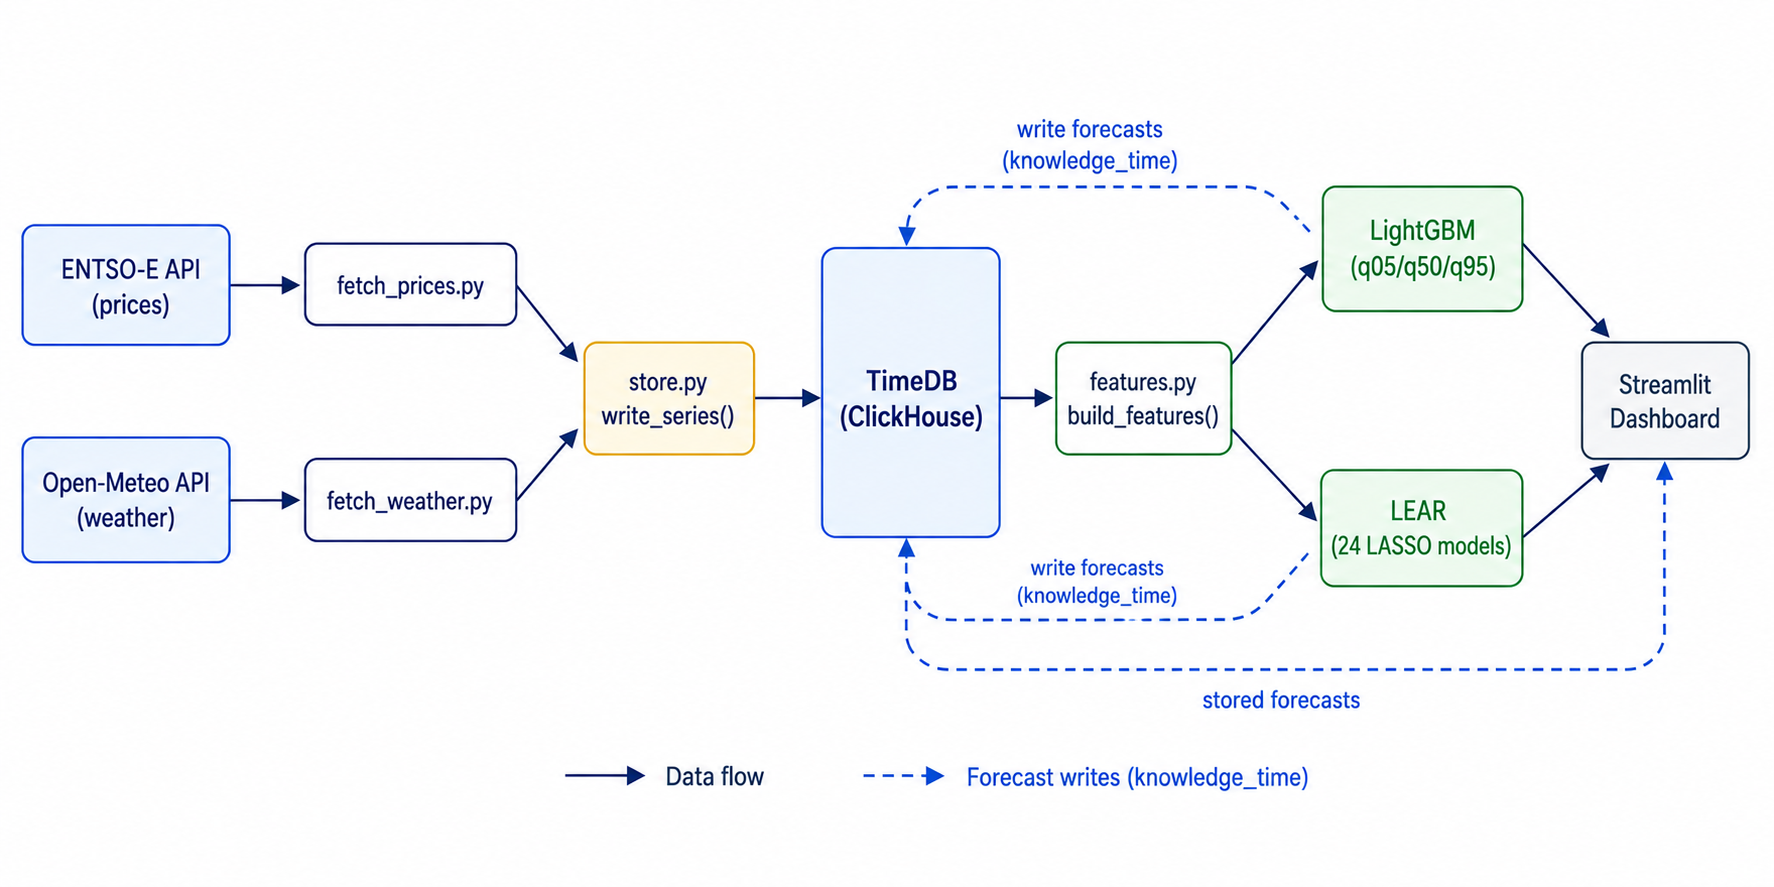
\includegraphics[width=\linewidth]{images/System_Architecture.png}
\caption{Full system architecture. Solid arrows = data flow. Dashed arrows = forecast
writes back to TimeDB (bitemporal storage).}
\label{fig:architecture}
\end{figure}

\section{Technology Stack}

\begin{center}
\begin{tabularx}{\linewidth}{llX}
\toprule
\textbf{Component} & \textbf{Technology} & \textbf{Why} \\
\midrule
Language        & Python 3.12          & Modern, async-ready, best ML ecosystem \\
Database        & ClickHouse 24.3      & Columnar OLAP, fast on time-series \\
Bitemporal ORM  & TimeDB 0.5.0         & Adds valid/knowledge time to ClickHouse \\
Forecasting     & LightGBM 4.x         & Fast, robust gradient boosting \\
Benchmark       & scikit-learn (LASSO) & LEAR model via LassoCV \\
Dashboard       & Streamlit            & Fast Python-native dashboards \\
Containerisation & Docker Compose      & Reproducible ClickHouse setup \\
Data viz        & Plotly               & Interactive charts in Streamlit \\
Prices API      & entsoe-py            & Python client for ENTSO-E \\
Weather API     & openmeteo-requests   & Free, no-key weather archive \\
\bottomrule
\end{tabularx}
\end{center}

\section{Project Directory Structure}

\begin{codefile}{\$PROJECT\_ROOT/}
\footnotesize
\begin{verbatim}
SE3_electricity_price_forecast_v2/
│
├── db/
│   └── schema.py          # Series ID registry; TimeDB init
│
├── pipeline/
│   ├── fetch_prices.py    # ENTSO-E price fetcher → TimeDB
│   ├── fetch_weather.py   # Open-Meteo weather fetcher → TimeDB
│   ├── features.py        # Builds hourly feature matrix from TimeDB
│   └── store.py           # write_series() helper (wraps td.write)
│
├── ml/
│   ├── models/
│   │   ├── lgbm.py        # LightGBM quantile regression (q05/q50/q95)
│   │   └── lear.py        # LEAR: 24 hourly LASSO models
│   ├── train.py           # Main training script + log + TimeDB writes
│   └── evaluate.py        # Walk-forward eval + CRPS
│
├── dashboard/
│   └── app.py             # Streamlit 6-tab dashboard
│
├── model/                 # Auto-managed by train.py
│   ├── MODEL_LOG.md       # Training run history (auto-appended)
│   ├── metrics.json       # Latest holdout metrics
│   ├── trained_at.json    # Training cache timestamp
│   ├── lgbm_q05/q50/q95.pkl
│   └── lear_h00...h23.pkl
│
├── docker-compose.yml     # ClickHouse container
├── .env / .env.example    # ENTSOE_API_KEY, TIMEDB_CH_URL
└── docs/
    └── SE3_Project_Textbook.tex   ← you are here
\end{verbatim}
\end{codefile}

% ═══════════════════════════════════════════════════════════════
\chapter{Data Sources}\label{ch:data}
% ═══════════════════════════════════════════════════════════════

\begin{chapterintro}
\sffamily\small\textbf{What you will learn:} Where the price data and weather data
come from, what we fetch, how we fetch it, and what the raw data looks like.
\end{chapterintro}

\section{ENTSO-E --- Electricity Prices}

\textbf{ENTSO-E} (European Network of Transmission System Operators for Electricity) is
the organisation that aggregates data from all European TSOs. Their Transparency Platform
publishes day-ahead prices for every European bidding zone.

\begin{keyidea}
We use the \textbf{entsoe-py} Python library to query ENTSO-E's REST API.
You need a free API key from \url{https://transparency.entsoe.eu}.
Store it in \code{.env} as \code{ENTSOE\_API\_KEY=your-key}.
\end{keyidea}

\textbf{What we fetch:} Day-ahead auction clearing prices for SE3, hourly, in EUR/MWh.
Zone EIC code: \code{10Y1001A1001A46L}.

\textbf{Data volume:} 71,967 rows from 2020-01-01 to 2026-05-13.

\begin{codefile}{pipeline/fetch\_prices.py --- full file}
\footnotesize
\begin{minted}{python}
SE3_ZONE = "10Y1001A1001A46L"          # EIC code for SE3 bidding zone

def fetch_prices(start, end):
    api_key = os.environ["ENTSOE_API_KEY"]
    client  = EntsoePandasClient(api_key=api_key)

    # Returns a pandas Series indexed by UTC timestamps
    series = client.query_day_ahead_prices(
        SE3_ZONE,
        start=pd.Timestamp(start),
        end=pd.Timestamp(end),
    )

    df = series.reset_index()
    df.columns = ["valid_time", "value"]           # tidy format for TimeDB
    df["valid_time"] = pd.to_datetime(df["valid_time"], utc=True)
    return df.dropna(subset=["value"])

def sync_prices(start, end):
    td = init_schema()
    df = fetch_prices(start, end)
    write_series(td, SERIES["prices_raw"], df, retention="forever")
    return len(df)
\end{minted}
\end{codefile}

\textbf{Run command:}
\begin{minted}{bash}
python -m pipeline.fetch_prices
\end{minted}

\section{Open-Meteo --- Weather Data}

\textbf{Open-Meteo} is a free, open-source weather API with no API key required.
It provides hourly historical and forecast weather data worldwide.

\textbf{Location:} Stockholm, Sweden --- latitude 59.33°N, longitude 18.07°E.
This is a reasonable proxy for SE3's population-weighted demand centre.

\textbf{What we fetch (3 variables):}

\begin{center}
\begin{tabular}{lll}
\toprule
\textbf{API variable} & \textbf{Our name} & \textbf{Why} \\
\midrule
\code{temperature\_2m}      & \code{temperature}   & Drives heating/cooling demand \\
\code{wind\_speed\_10m}     & \code{wind\_speed}   & Wind generation supply \\
\code{shortwave\_radiation} & \code{irradiance}    & Solar generation supply \\
\bottomrule
\end{tabular}
\end{center}

\begin{codefile}{pipeline/fetch\_weather.py --- key logic}
\begin{minted}{python}
_VARIABLES = ["temperature_2m", "wind_speed_10m", "shortwave_radiation"]
_SERIES_MAP = {
    "temperature_2m":      SERIES["weather_temperature"],   # ID 10
    "wind_speed_10m":      SERIES["weather_wind_speed"],    # ID 11
    "shortwave_radiation": SERIES["weather_irradiance"],    # ID 12
}

# Uses requests-cache (avoids re-fetching same dates) + retry (handles API blips)
def _build_client():
    cache   = requests_cache.CachedSession(".weather_cache", expire_after=3600)
    session = retry(cache, retries=5, backoff_factor=0.2)
    return openmeteo_requests.Client(session=session)

def fetch_weather(start, end):
    params = {
        "latitude": SE3_LAT,   "longitude": SE3_LON,
        "hourly":   _VARIABLES,
        "start_date": start.date().isoformat(),
        "end_date":   end.date().isoformat(),
        "timezone": "UTC",     "wind_speed_unit": "ms",
    }
    responses = client.weather_api(
        "https://archive-api.open-meteo.com/v1/archive", params=params
    )
    # Parse each variable → DataFrame[valid_time, value]
    ...
\end{minted}
\end{codefile}

\textbf{Run command:}
\begin{minted}{bash}
python -m pipeline.fetch_weather
\end{minted}

% ═══════════════════════════════════════════════════════════════
\chapter{Storage: TimeDB and Bitemporality}\label{ch:timedb}
% ═══════════════════════════════════════════════════════════════

\begin{chapterintro}
\sffamily\small\textbf{What you will learn:} What ClickHouse is, what TimeDB adds to
it, the bitemporal data model (the most important architectural concept in this project),
how to read and write data, and the retention bug we found and fixed.
\end{chapterintro}

\section{ClickHouse}

ClickHouse is a \textbf{column-oriented} OLAP database. Unlike row-oriented databases
(PostgreSQL, MySQL) that store data row-by-row, ClickHouse stores each column separately.
For time-series queries like \emph{``give me all prices from Jan to Mar''}, this means
reading only the \code{value} column --- not touching unrelated columns at all.
This makes it 10--100$\times$ faster than row stores for analytical queries.

We run ClickHouse locally via Docker:
\begin{minted}{bash}
docker-compose up -d        # start ClickHouse on ports 8123 (HTTP) and 9000 (TCP)
docker-compose down         # stop
\end{minted}

\section{TimeDB --- The Bitemporal Layer}

TimeDB is built \textbf{on top of} ClickHouse. It adds a single powerful concept:
\textbf{bitemporality}. Every row has two timestamps instead of one:

\begin{keyidea}
\begin{itemize}[noitemsep]
  \item \textbf{\code{valid\_time}}: \emph{When the event occurs in the real world.}
    Example: the SE3 price at 14:00 on 7 May 2026.
  \item \textbf{\code{knowledge\_time}}: \emph{When we learned or recorded it.}
    Example: the model produced this forecast on 13 May 2026 at 19:38 UTC.
\end{itemize}
\end{keyidea}

\subsection{The Bitemporal Grid}

Visualise a 2-dimensional plane where the x-axis is \code{valid\_time} and the y-axis
is \code{knowledge\_time}. Each data point is a square on this grid:

\begin{figure}[H]
\centering
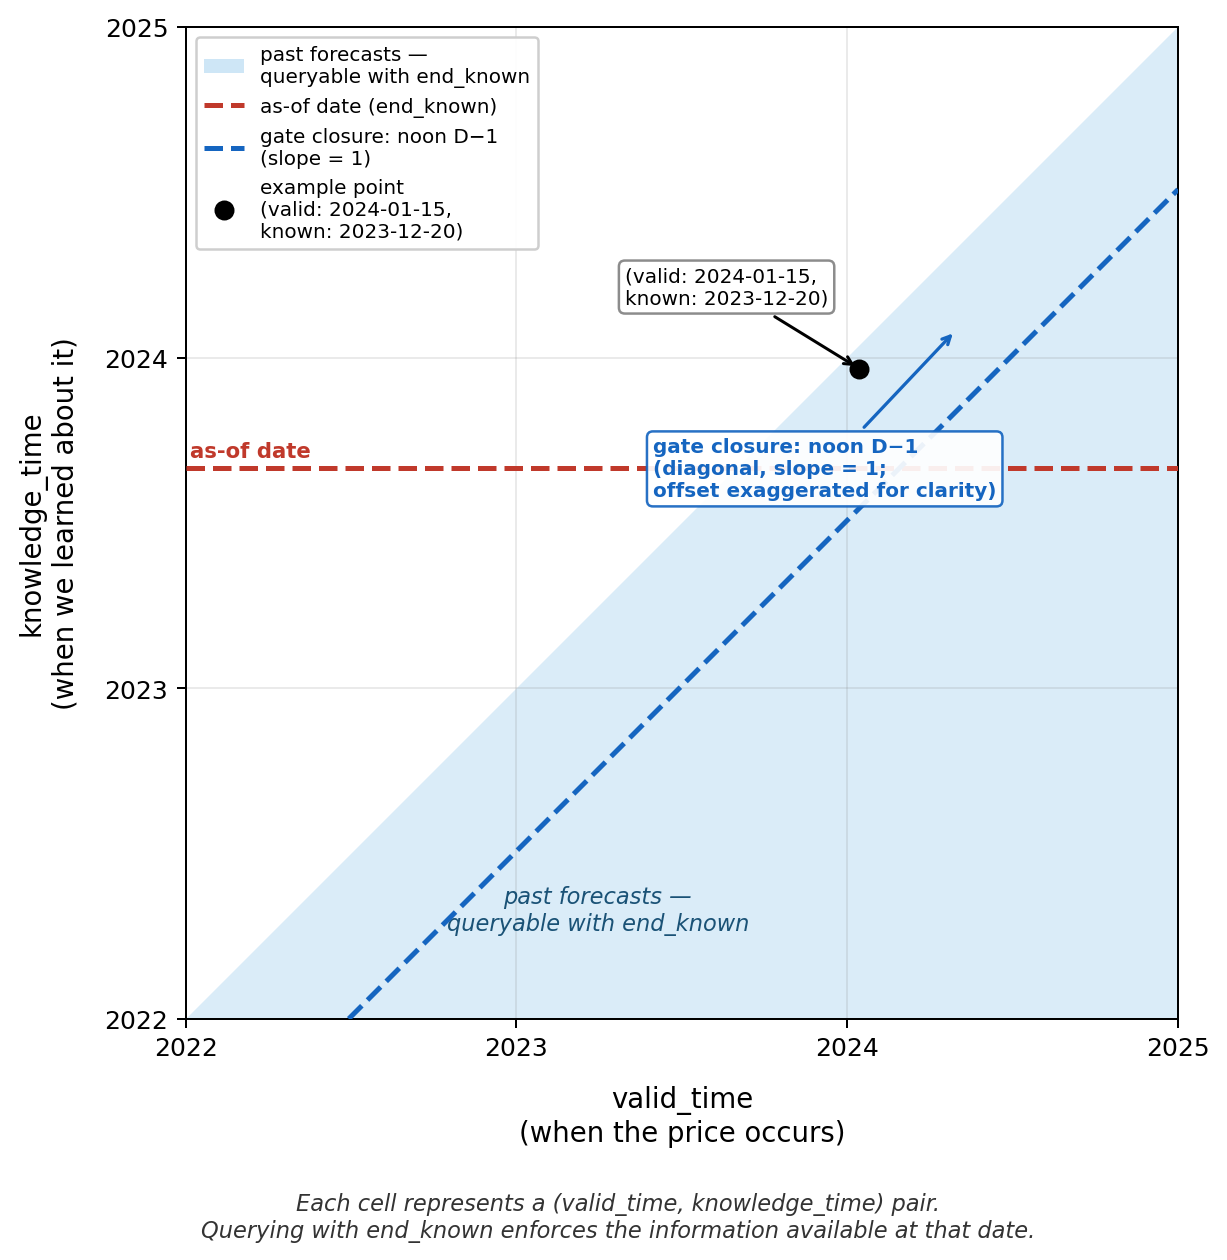
\includegraphics[width=0.82\linewidth]{images/Bitemporal_Grid_corrected.png}
\caption{The bitemporal grid. An as-of query with \code{end\_known=T} (red dashed line)
only returns data from training runs with \code{knowledge\_time < T}. Run 2's forecasts
are invisible to this query --- they didn't exist yet.}
\label{fig:bitemporal}
\end{figure}

\subsection{Why This Matters for Backtesting}

Without bitemporality, backtesting is subtly dishonest. If you train a model today on
data up to today, then evaluate it on data from 3 months ago, you are using a model
that was trained \emph{after} the evaluation period --- it has seen the future.

With TimeDB, you can ask: \emph{``What did the model predict for 7 May at 14:00,
using only the model that existed at noon on 6 May (gate closure)?''} This is
provably look-ahead-free.

\section{The Series ID Registry}

TimeDB identifies every time series by an integer \code{series\_id}.
We manage these in \filepath{db/schema.py}:

\begin{codefile}{db/schema.py --- Series registry}
\begin{minted}{python}
SERIES = {
    "prices_raw":         1,   # ENTSO-E day-ahead prices (EUR/MWh)
    "weather_temperature": 10, # Temperature (°C)
    "weather_wind_speed":  11, # Wind speed (m/s)
    "weather_irradiance":  12, # Shortwave radiation (W/m²)
    "lgbm_q05": 20,            # LightGBM 5th percentile forecast
    "lgbm_q50": 21,            # LightGBM median forecast
    "lgbm_q95": 22,            # LightGBM 95th percentile forecast
    "lear_q05": 30,            # LEAR 5th percentile
    "lear_q50": 31,            # LEAR median
    "lear_q95": 32,            # LEAR 95th percentile
}
\end{minted}
\end{codefile}

\section{TimeDB API Quick Reference}

\begin{center}
\begin{tabularx}{\linewidth}{lX}
\toprule
\textbf{Call} & \textbf{What it does} \\
\midrule
\code{td.write(df, retention, knowledge\_time)} & Write rows; \code{retention="forever"} for all our data \\
\code{td.read(series\_ids, retention)} & Read latest known value per \code{valid\_time} \\
\code{td.read(series\_ids, end\_known=T)} & As-of query: only rows where \code{knowledge\_time < T} \\
\code{td.read(include\_knowledge\_time=True)} & Returns the \code{knowledge\_time} column \\
\code{td.read\_relative(days\_ahead=1, time\_of\_day=time(12,0))} & Gate-closure backtest \\
\bottomrule
\end{tabularx}
\end{center}

\section{The Retention TTL Bug}

\begin{warningbox}
\textbf{What happened:} We initially wrote all data with \code{retention="medium"}.
ClickHouse's medium tier has a \textbf{1095-day (3-year) TTL from \code{valid\_time}}.
This silently deleted all data before May 2023 --- we lost 2020, 2021, and 2022 entirely.

\textbf{Symptom:} Only 23,943 labelled training rows instead of the expected 53,000+.
Only 45\% of feature rows had a matching price.

\textbf{Fix:} Changed all \code{write\_series()} calls to \code{retention="forever"}.
Re-fetched all data from 2020-01-01. Training set grew to 53,635 rows (100\% labelled).
\end{warningbox}

% ═══════════════════════════════════════════════════════════════
\chapter{Data Pipeline}\label{ch:pipeline}
% ═══════════════════════════════════════════════════════════════

\begin{chapterintro}
\sffamily\small\textbf{What you will learn:} How data flows from external APIs into
TimeDB, the \code{write\_series()} helper, and every command needed to keep the data
up to date.
\end{chapterintro}

\section{Pipeline Overview}

\begin{figure}[H]
\centering
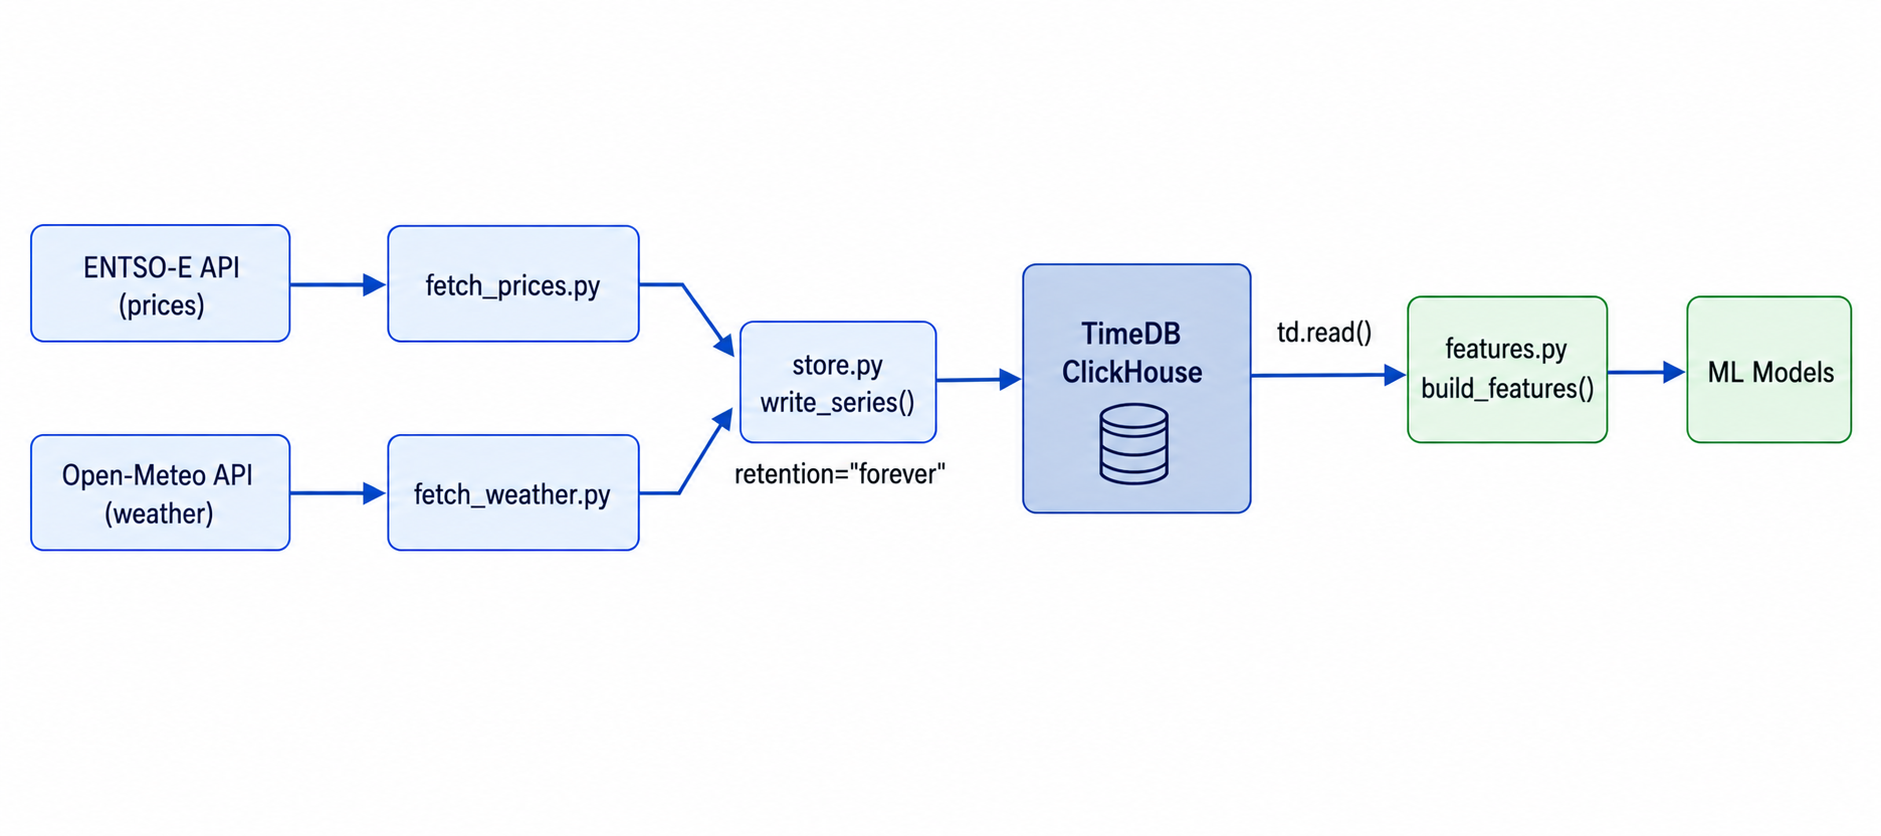
\includegraphics[width=\linewidth]{images/Pipeline_Overview.png}
\caption{Data pipeline flow from external APIs to the feature matrix.}
\end{figure}

\section{The write\_series() Helper}

\begin{codefile}{pipeline/store.py --- full file}
\begin{minted}{python}
def write_series(td, series_id, df, *, retention="forever", knowledge_time=None):
    """Write a tidy DataFrame into TimeDB for a given series_id.

    df must have columns: valid_time (UTC datetime) and value (float).
    series_id is added here before writing.
    """
    df = df.copy()
    df["series_id"] = series_id          # tag each row with the series integer ID
    td.write(df, retention=retention, knowledge_time=knowledge_time)
\end{minted}
\end{codefile}

The \code{knowledge\_time} parameter defaults to \code{None}, meaning TimeDB uses
\emph{now} as the knowledge time. For forecast writes in \code{train.py}, we pass
the exact training run timestamp so the bitemporal record is accurate.

\section{Commands Reference}

\begin{center}
\begin{tabularx}{\linewidth}{lX}
\toprule
\textbf{Command} & \textbf{Effect} \\
\midrule
\code{python -m pipeline.fetch\_prices}  & Fetch prices from 2020-01-01 to now \\
\code{python -m pipeline.fetch\_weather} & Fetch weather (temperature, wind, irradiance) \\
\code{python -m ml.train}                & Train models (skips if $<7$ days since last run) \\
\code{python -m ml.train --force}        & Train regardless of cache \\
\code{.venv/bin/streamlit run dashboard/app.py} & Launch dashboard \\
\bottomrule
\end{tabularx}
\end{center}

% ═══════════════════════════════════════════════════════════════
\chapter{Feature Engineering}\label{ch:features}
% ═══════════════════════════════════════════════════════════════

\begin{chapterintro}
\sffamily\small\textbf{What you will learn:} Every single feature in the model --- what
it is, why it was chosen (the electricity market intuition), and exactly how it is
computed in \filepath{pipeline/features.py}.
\end{chapterintro}

\section{Overview: The Feature Map}

\begin{figure}[H]
\centering
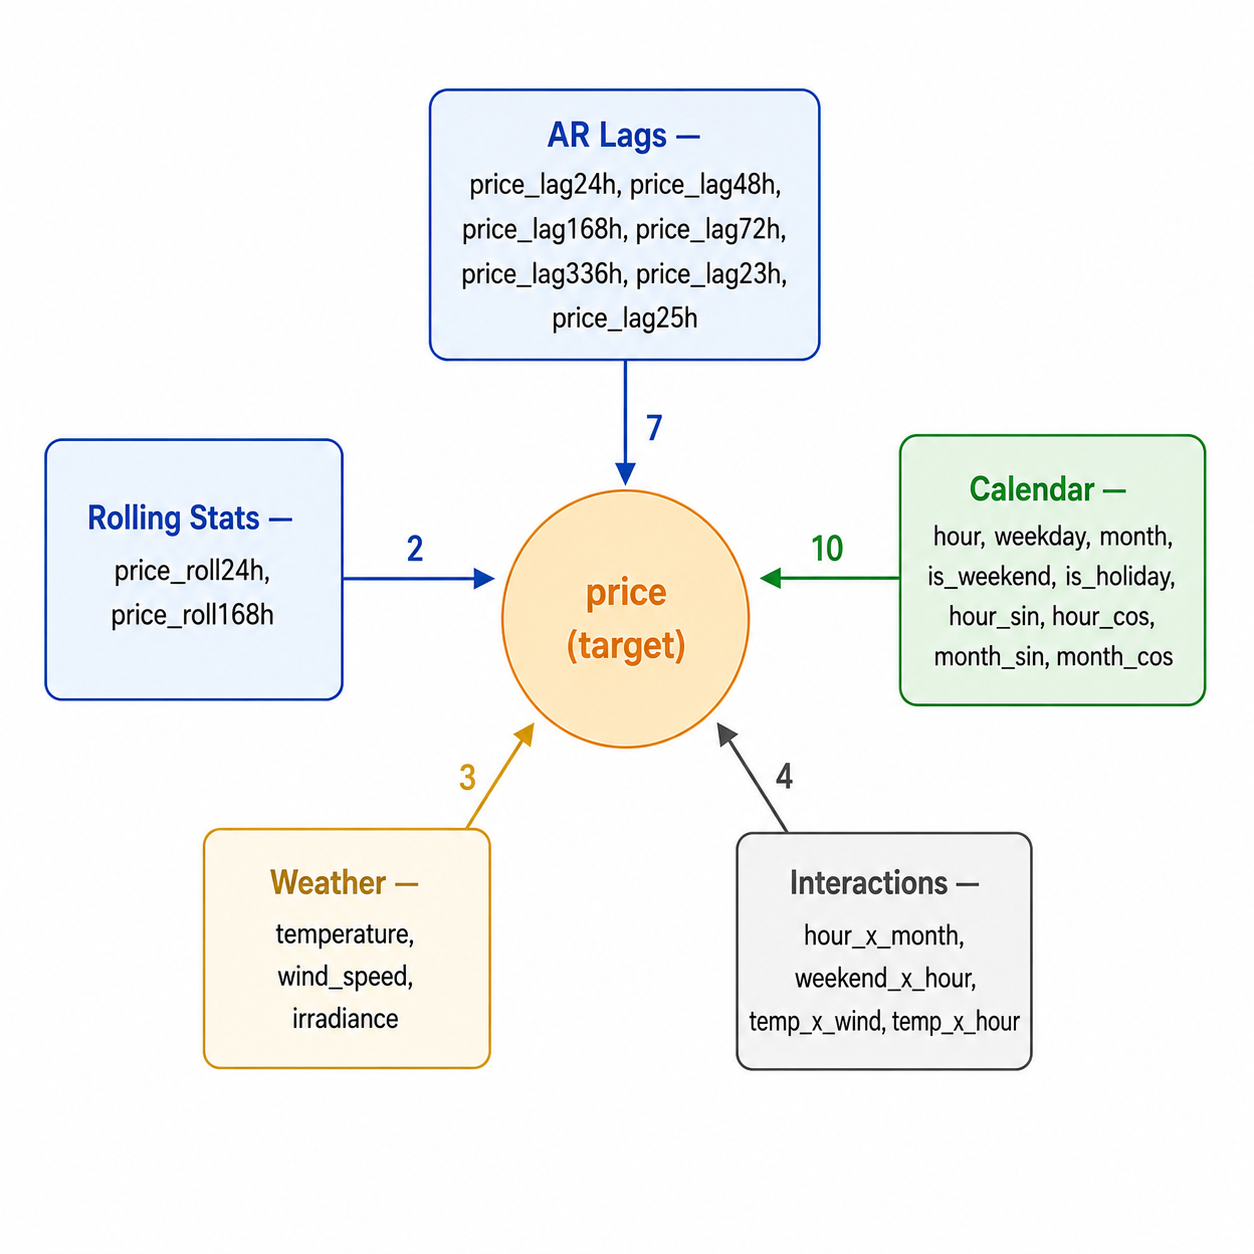
\includegraphics[width=0.85\linewidth]{images/Feature_Map_Overview.png}
\caption{All 26 features feeding into the models, grouped by type.}
\label{fig:featuremap}
\end{figure}

\section{Autoregressive (AR) Price Lags}

\begin{keyidea}
The best predictor of tomorrow's price at 14:00 is \emph{yesterday's} price at 14:00.
This is the autoregressive (AR) structure of electricity prices: they are strongly
correlated with their own past values at multiples of 24 hours.
\end{keyidea}

We compute 7 lags. Here is the full rationale for each:

\begin{center}
\begin{tabularx}{\linewidth}{llX}
\toprule
\textbf{Feature} & \textbf{Hours} & \textbf{Market rationale} \\
\midrule
\code{price\_lag24h}  & 24  & Same hour yesterday --- single most important feature. Strong daily autocorrelation. \\
\code{price\_lag48h}  & 48  & Same hour 2 days ago. Yesterday may have been unusual; 48h gives a second reference. \\
\code{price\_lag168h} & 168 & Same hour 1 week ago. Captures weekly seasonality (Mon/Fri vs Tue--Thu differ). \\
\code{price\_lag72h}  & 72  & Same hour 3 days ago. Mon prices correlate with Thu of previous week. \\
\code{price\_lag336h} & 336 & Same hour 2 weeks ago. \textbf{Nuclear outage cycles}: SE3 nuclear plants have roughly fortnightly maintenance patterns. \\
\code{price\_lag23h}  & 23  & Adjacent hour (h$-$1) from yesterday. Provides cross-hour context so models for adjacent hours share information. \textbf{v2 addition.} \\
\code{price\_lag25h}  & 25  & Adjacent hour (h$+$1) from yesterday. Same rationale. \textbf{v2 addition.} \\
\bottomrule
\end{tabularx}
\end{center}

\begin{codefile}{pipeline/features.py, lines 76--77}
\begin{minted}{python}
lags     = [23, 24, 25, 48, 72, 168, 336]
lag_feats = [_lag(price, h) for h in lags]   # _lag(s, h) = s.shift(h)
\end{minted}
\end{codefile}

\section{Rolling Statistics --- Leakage-Free Design}

Rolling means capture the recent \emph{level} of prices (are we in a high-price regime
or a low-price regime?). However, there is a critical data leakage trap:

\begin{warningbox}
\textbf{Data leakage in rolling means:} If you compute \code{price.rolling(24).mean()}
and use it as a feature to predict \code{price[t]}, the rolling mean includes
\code{price[t]} itself and prices from hours $t-1, t-2, \ldots$ --- none of which
would be available at gate closure (noon D-1).

\textbf{Fix:} Always compute rolling means on \code{price.shift(24)}, not on
the raw price series. This ensures the rolling mean only uses prices from at least
24 hours ago.
\end{warningbox}

The correct computation, for a 24-hour rolling mean:
\[
  \text{roll}_{24}(t) = \frac{1}{24}\sum_{i=1}^{24} p_{t-24-i}
  = \frac{1}{24}\left(p_{t-25} + p_{t-26} + \cdots + p_{t-48}\right)
\]

\begin{codefile}{pipeline/features.py, lines 80--84}
\begin{minted}{python}
price_lag24 = price.shift(24)          # shift first! Avoids leakage.
roll_feats = [
    _rolling_mean(price_lag24.rename("price"), 24).rename("price_roll24h"),
    _rolling_mean(price_lag24.rename("price"), 168).rename("price_roll168h"),
]
\end{minted}
\end{codefile}

\section{Calendar Features}

\subsection{Raw Calendar}

\begin{codefile}{pipeline/features.py, lines 88--95}
\begin{minted}{python}
cal["hour"]       = idx.hour          # 0-23
cal["weekday"]    = idx.dayofweek     # 0=Monday, 6=Sunday
cal["month"]      = idx.month         # 1-12
cal["is_weekend"] = (idx.dayofweek >= 5).astype(int)   # Sat/Sun = 1
cal["is_holiday"] = idx.normalize().map(               # Swedish public holidays
    lambda d: int(d.date() in SE_HOLIDAYS))
cal["hour_of_week"] = idx.dayofweek * 24 + idx.hour   # 0-167
\end{minted}
\end{codefile}

\subsection{Cyclical Encoding}

\begin{keyidea}
\textbf{Why not just use the raw integer for hour?} The problem: hour 23 and hour 0 are
adjacent in time but numerically far apart (23 vs 0). A tree model treats them as distant.
We need the feature space to ``wrap around'' like a clock.

\textbf{Solution:} Encode each cyclic variable as a pair $(\sin, \cos)$:
\[
  h_{\sin}(t) = \sin\!\left(\frac{2\pi \cdot \text{hour}(t)}{24}\right), \qquad
  h_{\cos}(t) = \cos\!\left(\frac{2\pi \cdot \text{hour}(t)}{24}\right)
\]

Hours 0 and 23 now have a small angular distance. The same trick applies to weekday
(period 7) and month (period 12).
\end{keyidea}

\begin{align}
  \text{hour\_sin}    &= \sin\!\left(\frac{2\pi \cdot \text{hour}}{24}\right) &
  \text{hour\_cos}    &= \cos\!\left(\frac{2\pi \cdot \text{hour}}{24}\right) \\
  \text{weekday\_sin} &= \sin\!\left(\frac{2\pi \cdot \text{weekday}}{7}\right) &
  \text{weekday\_cos} &= \cos\!\left(\frac{2\pi \cdot \text{weekday}}{7}\right) \\
  \text{month\_sin}   &= \sin\!\left(\frac{2\pi (\text{month}-1)}{12}\right) &
  \text{month\_cos}   &= \cos\!\left(\frac{2\pi (\text{month}-1)}{12}\right)
\end{align}

\section{Interaction Features (v2 Additions)}

Interaction features let the model learn that the \emph{effect} of one variable
depends on the value of another. All four were added in v2.

\begin{center}
\begin{tabularx}{\linewidth}{llX}
\toprule
\textbf{Feature} & \textbf{Formula} & \textbf{Why} \\
\midrule
\code{hour\_x\_month}   & $\text{hour} \times \text{month}$   & Evening peak is longer and higher in winter (month 12) than summer (month 6). This term captures the seasonal time-of-day shape. \\
\code{weekend\_x\_hour} & $\text{is\_weekend} \times h_{\sin}$& Weekend daily pattern peaks later and at lower amplitude. The product encodes both the weekend flag and the time-of-day together. \\
\code{temp\_x\_hour}    & $\text{temperature} \times \text{hour}$ & Cold mornings create larger demand spikes at morning peak hours. Warm summer afternoons suppress afternoon demand. \\
\code{temp\_x\_wind}    & $\text{temperature} \times \text{wind\_speed}$ & Cold + windy feels colder (wind chill): heating demand spikes more than either factor alone would suggest. \\
\bottomrule
\end{tabularx}
\end{center}

\begin{codefile}{pipeline/features.py, lines 107--123}
\begin{minted}{python}
cal["hour_x_month"]   = cal["hour"] * cal["month"]
cal["weekend_x_hour"] = cal["is_weekend"] * cal["hour_sin"]
temp_x_wind = (temp * wind).rename("temp_x_wind")
temp_x_hour = (temp * cal["hour"]).rename("temp_x_hour")
\end{minted}
\end{codefile}

% ═══════════════════════════════════════════════════════════════
\chapter{Models}\label{ch:models}
% ═══════════════════════════════════════════════════════════════

\begin{chapterintro}
\sffamily\small\textbf{What you will learn:} How LightGBM quantile regression works
mathematically, every hyperparameter and why it was changed in v2, how LEAR works,
what LASSO does, and how prediction intervals are produced by both models.
\end{chapterintro}

\section{LightGBM --- Quantile Regression}

\subsection{Gradient Boosting Refresher}

LightGBM is a \textbf{gradient boosted decision tree} (GBDT) framework. It builds an
ensemble of trees sequentially, where each new tree corrects the errors of all previous trees:

\[
  F_M(x) = \sum_{m=1}^{M} \eta \cdot h_m(x)
\]

where $h_m$ is the $m$-th decision tree, $\eta$ is the learning rate (0.03 in v2),
and $M$ is the total number of trees (up to 3000, controlled by early stopping).

\subsection{Quantile (Pinball) Loss}

Instead of the usual squared error $\mathcal{L} = (y - \hat{y})^2$, we use the
\textbf{pinball loss} (also called quantile loss) for a target quantile $\tau$:

\begin{keyidea}
\[
  \mathcal{L}_\tau(y, \hat{y}) = \begin{cases}
    \tau \cdot (y - \hat{y})       & \text{if } y \geq \hat{y} \quad \text{(underestimate)} \\
    (1-\tau) \cdot (\hat{y} - y)  & \text{if } y < \hat{y}  \quad \text{(overestimate)}
  \end{cases}
\]
\end{keyidea}

\begin{intuition}
For $\tau = 0.95$: underestimates are penalised 19$\times$ more heavily than overestimates.
So the model learns to predict high --- it becomes the upper bound (q95). For $\tau = 0.05$:
overestimates are penalised 19$\times$ more --- the model predicts low, giving the lower
bound (q05). For $\tau = 0.50$: equal penalty either side --- equivalent to minimising MAE,
giving the median forecast.
\end{intuition}

\subsection{Three Independent Models}

We train \textbf{three separate LightGBM models}, one per quantile:
\code{lgbm\_q05.pkl}, \code{lgbm\_q50.pkl}, \code{lgbm\_q95.pkl}.

\begin{figure}[H]
\centering
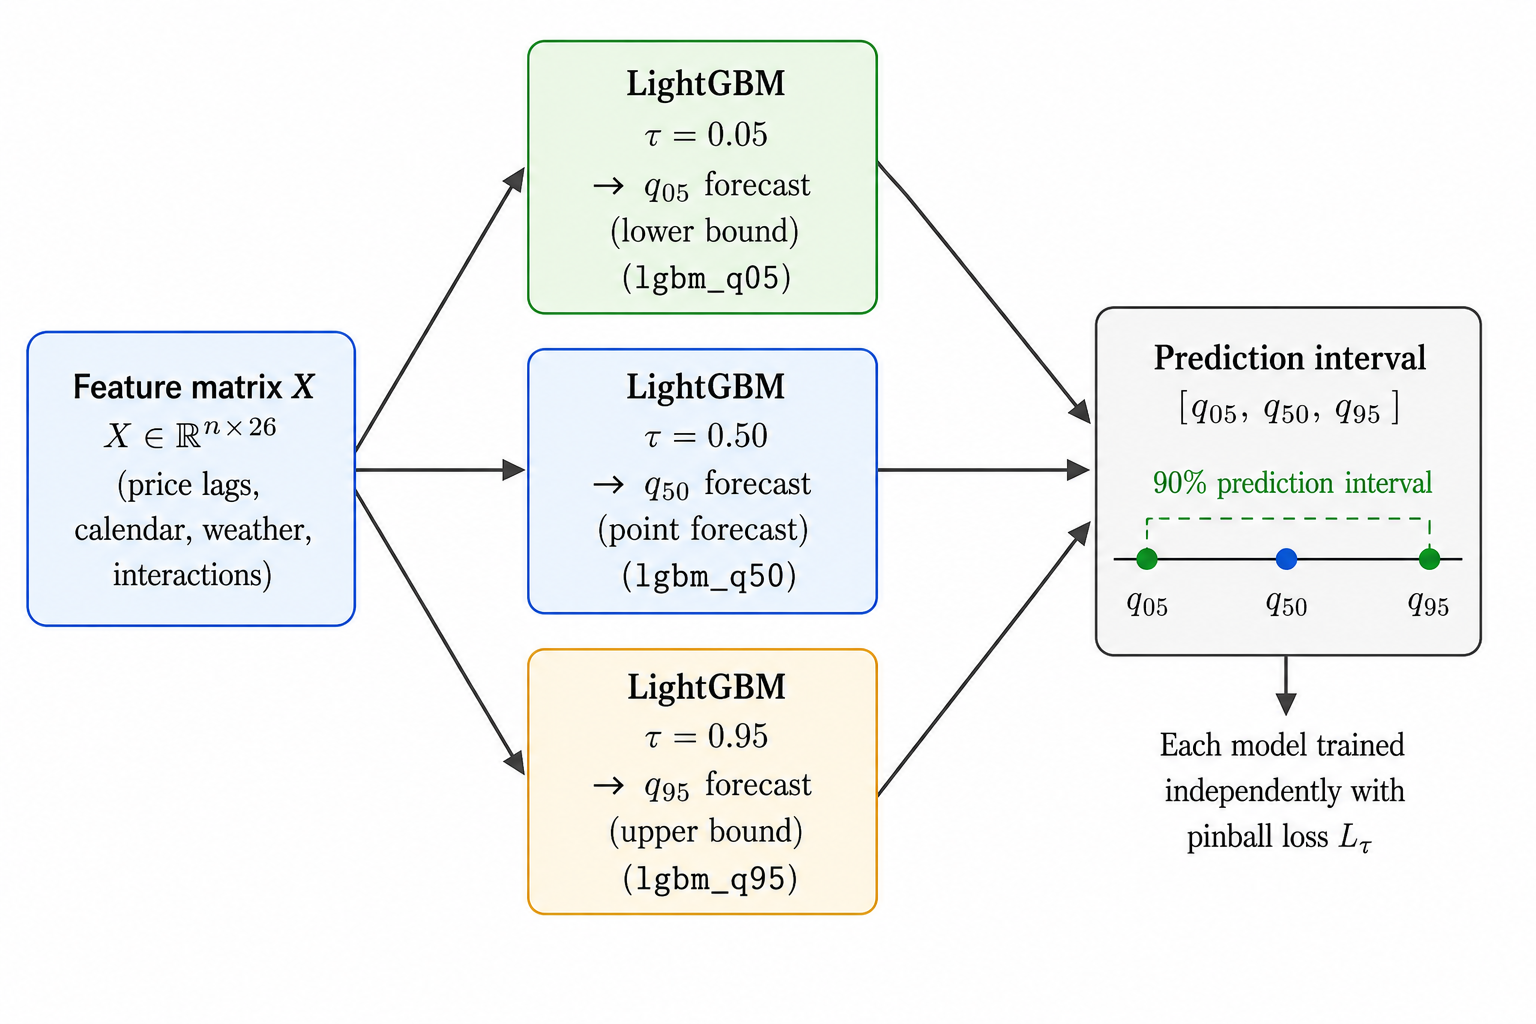
\includegraphics[width=0.78\linewidth]{images/LightGBM_models.png}
\caption{Three independent quantile models feed a single feature matrix.}
\end{figure}

\subsection{Hyperparameters: Before vs After v2}

\begin{center}
\begin{tabularx}{\linewidth}{lllX}
\toprule
\textbf{Parameter} & \textbf{Before} & \textbf{After} & \textbf{Why changed} \\
\midrule
\code{num\_leaves}        & 63   & 127  & More expressive trees; offset by stronger regularisation \\
\code{min\_child\_samples}& 20   & 50   & Primary anti-overfitting guard. Each leaf needs $\geq$50 samples (prevents fitting spike noise) \\
\code{colsample\_bytree}  & 0.8  & 0.6  & Feature-level bagging: each tree sees only 60\% of features $\rightarrow$ more diverse ensemble \\
\code{subsample}          & 0.8  & 0.7  & Row-level bagging: each tree trained on 70\% of rows \\
\code{reg\_alpha} (L1)    & 0.1  & 0.3  & Drives small feature weights to exactly zero \\
\code{reg\_lambda} (L2)   & 0.1  & 0.3  & Shrinks all weights $\rightarrow$ smoother predictions \\
\code{learning\_rate}     & 0.05 & 0.03 & Slower convergence $\rightarrow$ finer optimisation at cost of more trees \\
\code{n\_estimators}      & 1000 (fixed) & 3000 + early stopping & Actual count determined by validation \\
\bottomrule
\end{tabularx}
\end{center}

\subsection{Early Stopping}

We hold out the last 15\% of training rows (\code{VAL\_FRAC = 0.15}) as a validation
window. Training stops when validation quantile loss does not improve for 50 consecutive
rounds (\code{EARLY\_STOP\_N = 50}).

From MODEL\_LOG, the three models stopped at: \textbf{357, 391, 110} iterations
(out of a maximum of 3000). The q95 model stopped much earlier (110), suggesting
the upper bound is easier to learn than the lower bound.

\subsection{Recency Weighting}

Electricity market dynamics change over time (renewable penetration grows, demand
patterns shift). We weight recent observations more heavily using exponential decay:

\begin{keyidea}
\[
  w_i = \exp\!\left(-\frac{\ln 2 \cdot (T - t_i)}{H}\right), \qquad H = 365 \times 24 \text{ hours}
\]

where $T$ is the most recent timestamp, $t_i$ is the timestamp of observation $i$,
and $H$ is the half-life. With $H = 365 \times 24$, data from exactly one year ago
has weight $w = 0.5$ (half the weight of today's data).
\end{keyidea}

\begin{codefile}{ml/models/lgbm.py, lines 97--101}
\begin{minted}{python}
def _recency_weights(n):
    decay = np.exp(-np.log(2) * np.arange(n)[::-1] / WEIGHT_HALF_LIFE_HOURS)
    return decay / decay.mean()   # normalise: mean weight = 1
\end{minted}
\end{codefile}

% ── LEAR ─────────────────────────────────────────────────────
\section{LEAR --- LASSO Estimated AutoRegressive}

LEAR is the academic benchmark from
\textit{Lago et al. (2021), Applied Energy 293, 116983}. It is much simpler than
LightGBM but achieves competitive accuracy and serves as a calibration reference.

\subsection{One Model Per Hour}

LEAR trains \textbf{24 independent LASSO regression models}, one for each hour of
the day. Model for hour $h$ only trains on data where the hour of day is $h$, and
only predicts hour $h$ prices.

\begin{figure}[H]
\centering
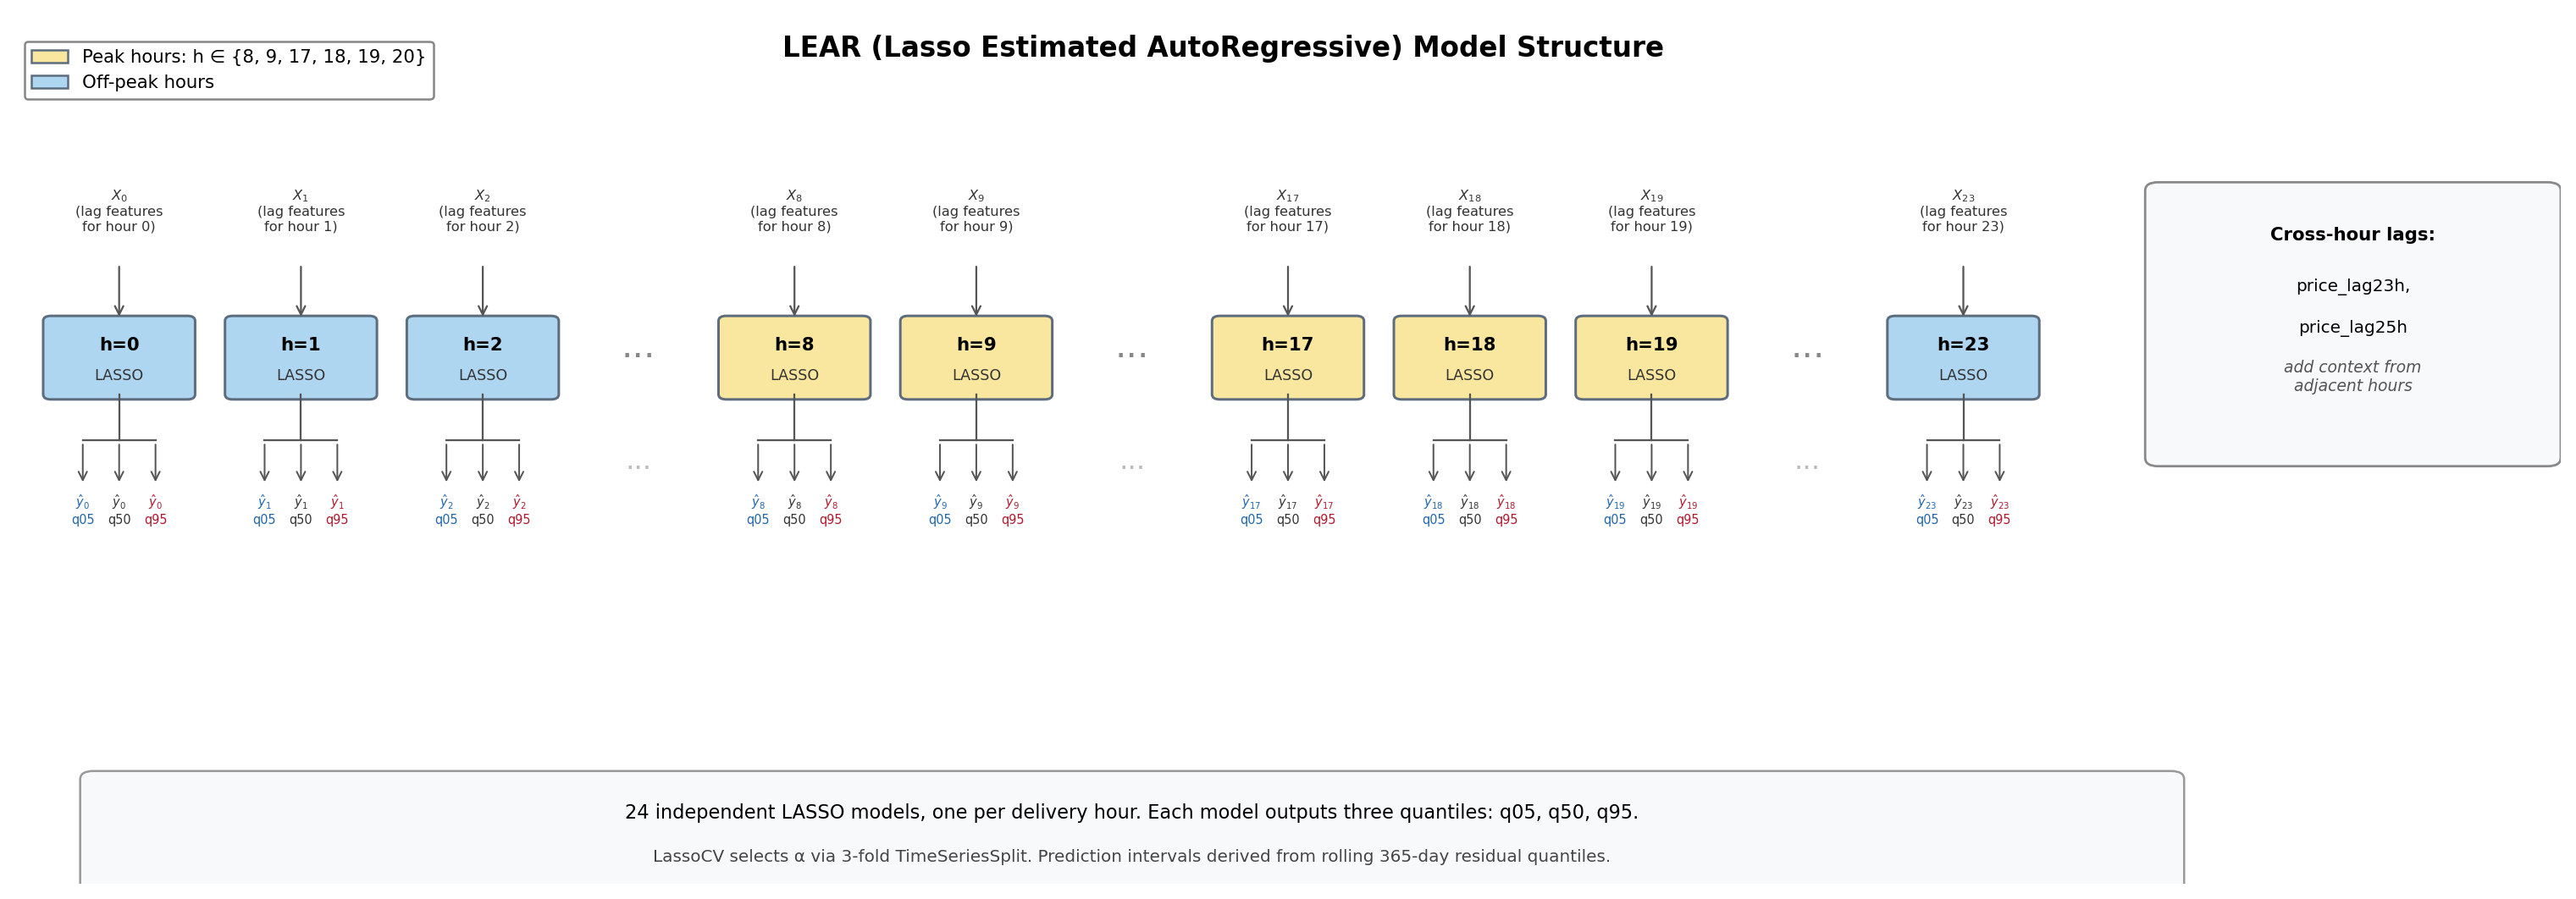
\includegraphics[width=\linewidth]{images/LASSO_models_corrected.png}
\caption{LEAR: 24 hourly LASSO models. Red arrows show the cross-hour lags added in v2
--- adjacent-hour prices from yesterday flow between models.}
\label{fig:lear}
\end{figure}

\subsection{LASSO Regression}

The core model for each hour $h$ is:
\begin{keyidea}
\[
  \hat{\boldsymbol{\beta}}_h = \arg\min_{\boldsymbol{\beta}} \left[
    \frac{1}{n_h}\|y_h - X_h\boldsymbol{\beta}\|_2^2 + \alpha\|\boldsymbol{\beta}\|_1
  \right]
\]
where $X_h$ is the feature matrix for hour $h$, $y_h$ is the vector of prices
at hour $h$, and $\alpha$ controls regularisation strength.
\end{keyidea}

The L1 penalty $\alpha\|\boldsymbol{\beta}\|_1 = \alpha\sum_j|\beta_j|$ drives
small coefficients to \emph{exactly} zero, performing automatic feature selection.
Features that are irrelevant for a specific hour get zeroed out.

\subsection{StandardScaler --- Why Required}

LASSO penalises coefficients by their \emph{magnitude}. If temperature is in the range
$[-20, +30]$ and \code{hour\_sin} is in $[-1, +1]$, an unscaled LASSO will unfairly
penalise the temperature coefficient more. We normalise every feature:

\[
  z_j = \frac{x_j - \mu_j}{\sigma_j}
\]

using \code{sklearn.preprocessing.StandardScaler} fitted on the training data only.

\subsection{LassoCV --- Data-Driven Alpha Selection}

\begin{warningbox}
\textbf{v1 used a fixed $\alpha = 0.001$} (the Lago et al. default). But the optimal
$\alpha$ varies by hour: late-night hours have simpler price dynamics (low $\alpha$)
while peak hours are noisier (higher $\alpha$ needed). Using a fixed value is suboptimal.
\end{warningbox}

In v2, we use \code{LassoCV} to select $\alpha$ via cross-validation from a grid:
$\alpha \in \{10^{-4}, 5\times10^{-4}, 10^{-3}, 5\times10^{-3}, 10^{-2}, 5\times10^{-2}, 10^{-1}, 5\times10^{-1}\}$

\textbf{TimeSeriesSplit} (3 folds) is used instead of random CV, because time ordering
must be preserved: you cannot train on future data to predict the past.

\begin{figure}[H]
\centering
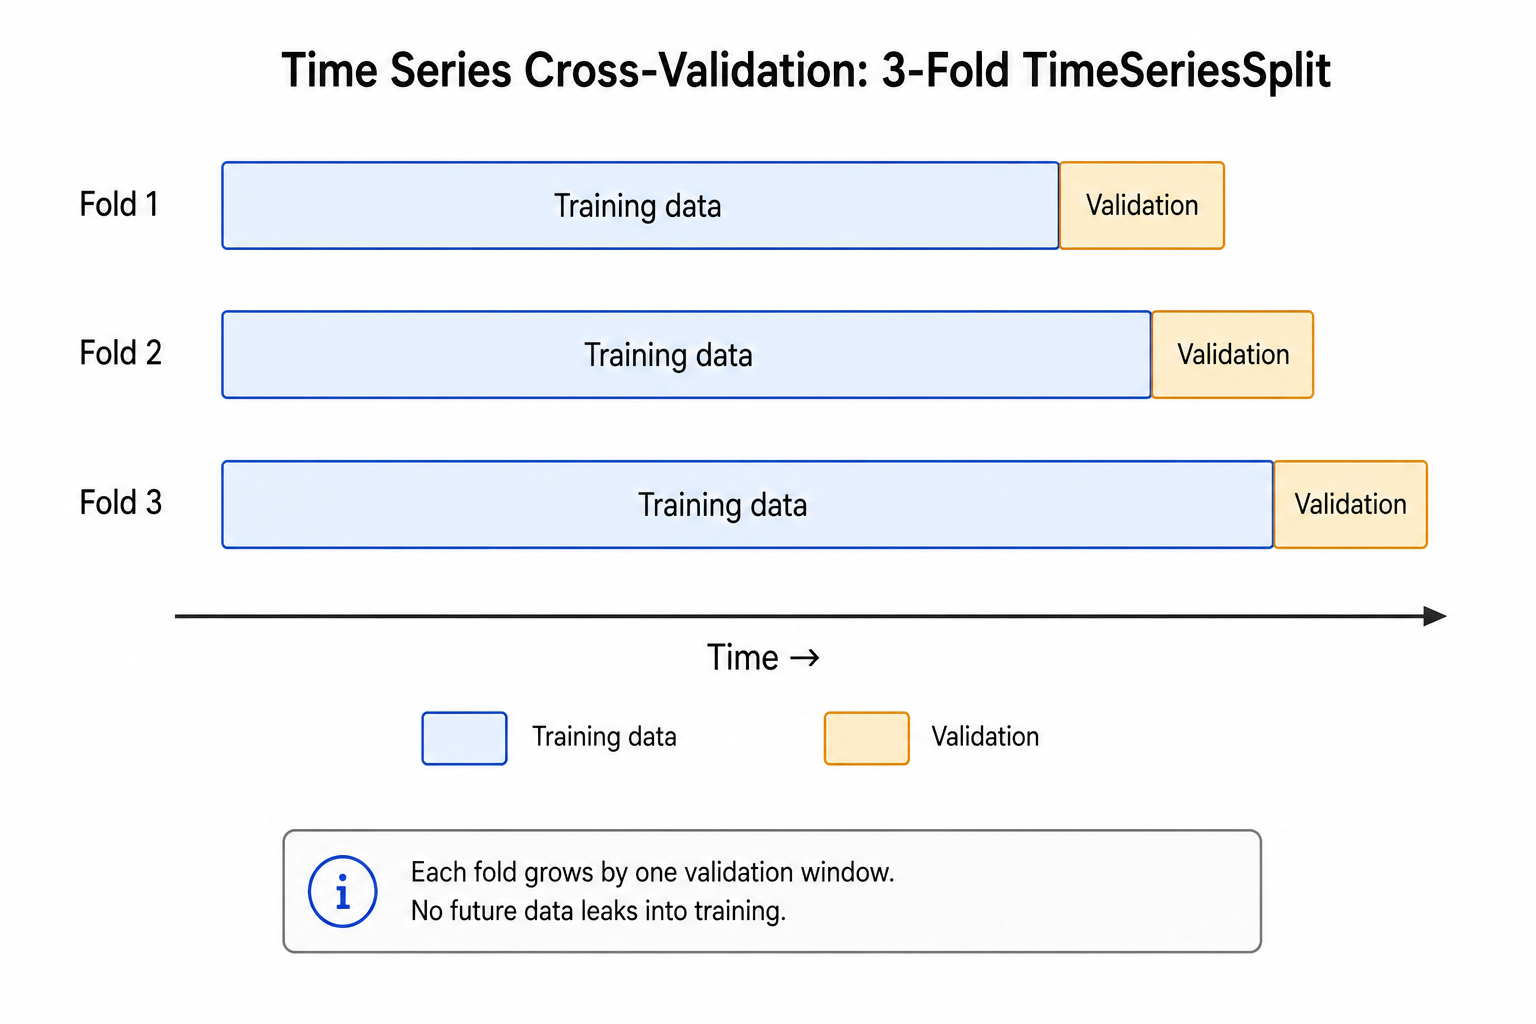
\includegraphics[width=0.70\linewidth]{images/TimeSeriesSplit.png}
\caption{TimeSeriesSplit(3): each fold's validation window is always \emph{after} its
training data. This prevents any look-ahead bias in alpha selection.}
\end{figure}

\subsection{Prediction Intervals for LEAR}

LASSO is a point forecast model. We add prediction intervals using the empirical
distribution of in-sample residuals:

\[
  \hat{r}_i = y_i - \hat{y}_i \qquad \text{(residual for training observation } i\text{)}
\]

\[
  \hat{q}_{0.05}(t) = \hat{y}(t) + Q_{0.05}(\hat{r}) \qquad
  \hat{q}_{0.95}(t) = \hat{y}(t) + Q_{0.95}(\hat{r})
\]

\textbf{v2 improvement}: we use only the \textbf{last 365 days} of residuals
(\code{RESID\_WINDOW = 365 * 24}). Older residuals reflect past volatility regimes
that no longer apply to today's market.

% ═══════════════════════════════════════════════════════════════
\chapter{Training Pipeline}\label{ch:training}
% ═══════════════════════════════════════════════════════════════

\begin{chapterintro}
\sffamily\small\textbf{What you will learn:} How \code{train.py} works end-to-end,
the 90-day holdout design, the training cache, and how forecasts are written to TimeDB.
\end{chapterintro}

\section{Training Flowchart}

\begin{figure}[H]
\centering
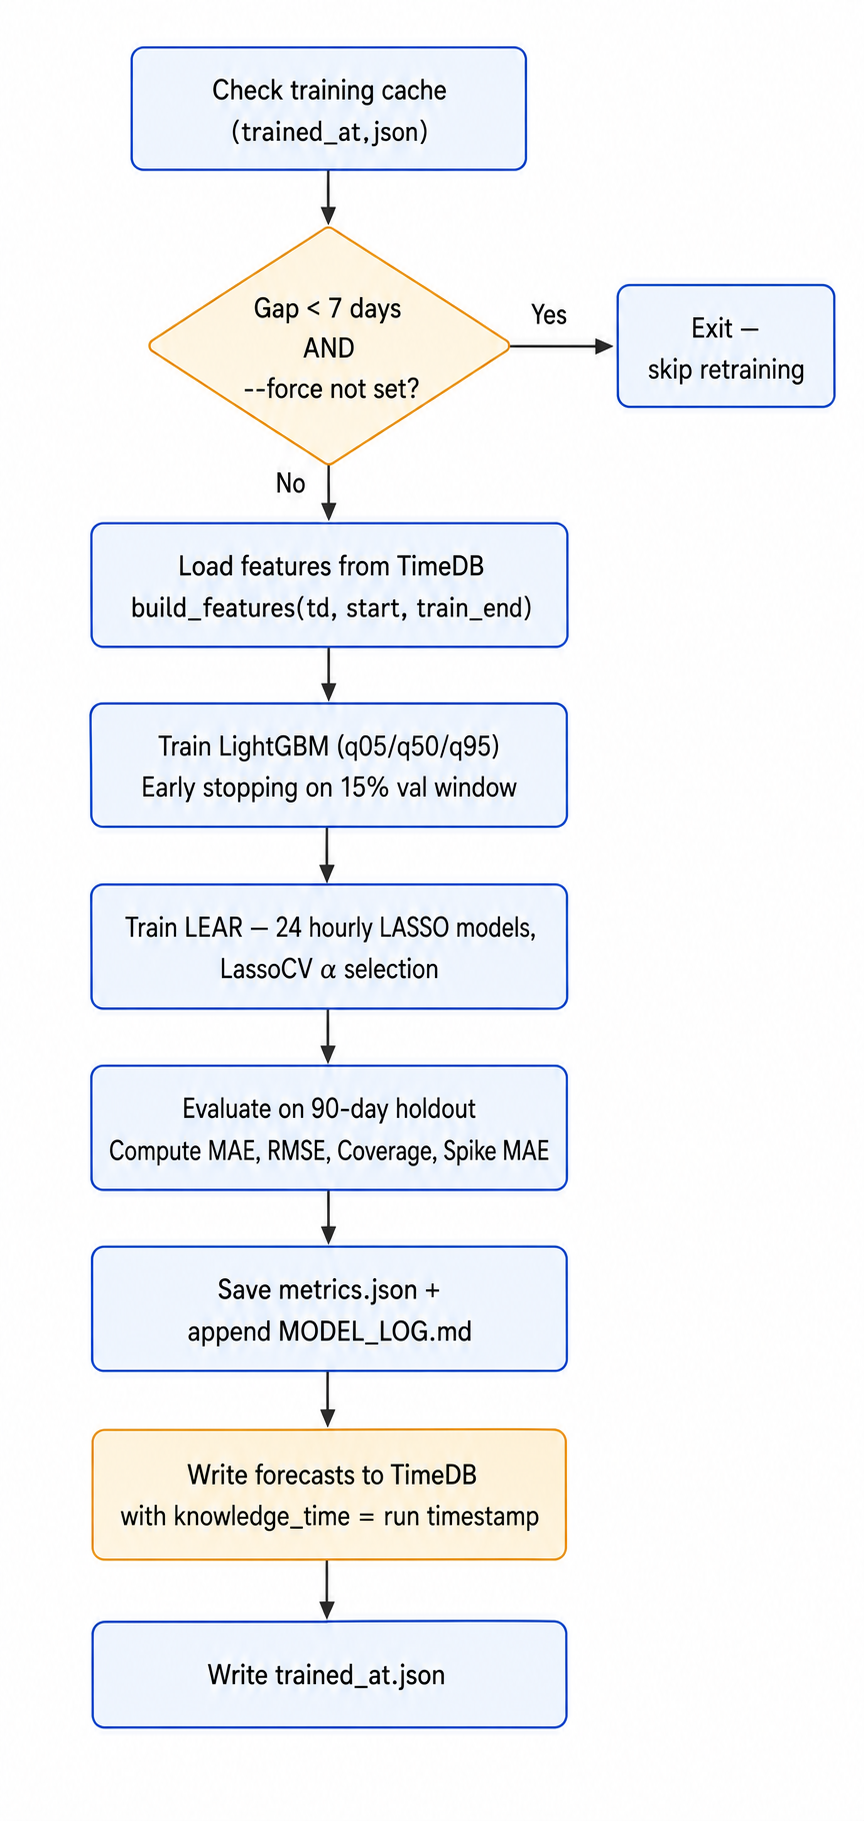
\includegraphics[width=0.60\linewidth]{images/Training_Flowchart.png}
\caption{Complete \code{ml/train.py} execution flow.}
\end{figure}

\section{The 90-Day Holdout}

The training period runs from 2020-01-01 to \code{train\_end = now - 90 days}.
The holdout is the last 90 days. \textbf{Why 90 days?}
\begin{itemize}
  \item Long enough to capture one full season's worth of variation
  \item Short enough to remain within the most recent market regime
  \item Matches what practitioners use for short-term forecasting model evaluation
\end{itemize}

\begin{warningbox}
\textbf{Never use random train/test splits for time-series.} A random split would
allow the model to train on May data and be evaluated on March data --- the model
has effectively ``seen the future''. Always split chronologically.
\end{warningbox}

\section{Training Cache}

\begin{codefile}{ml/train.py --- \_should\_skip\_training()}
\begin{minted}{python}
def _should_skip_training(td):
    # Requires: trained_at.json exists + model pickle files exist
    with open(MODEL_DIR / "trained_at.json") as f:
        info = json.load(f)
    trained_dt     = datetime.fromisoformat(info["trained_at"])
    latest_price   = td.read(series_ids=[SERIES["prices_raw"]],
                             retention="forever").to_pandas()
    latest_time    = pd.to_datetime(latest_price["valid_time"], utc=True).max()
    gap_days       = (latest_time - trained_dt).total_seconds() / 86_400
    return gap_days < 7    # skip if less than 7 days of new data
\end{minted}
\end{codefile}

Commands:
\begin{minted}{bash}
python -m ml.train           # auto-skip if < 7 days since last run
python -m ml.train --force   # retrain regardless
\end{minted}

\section{Writing Forecasts to TimeDB}

After evaluation, holdout predictions are written back to TimeDB with
\code{knowledge\_time = run\_kt} (the exact moment training finished):

\begin{codefile}{ml/train.py --- \_write\_forecasts\_to\_timedb()}
\begin{minted}{python}
mapping = [
    ("lgbm_q05", lgbm_val["lgbm_q05"]),
    ("lgbm_q50", lgbm_val["lgbm_q50"]),
    ("lgbm_q95", lgbm_val["lgbm_q95"]),
    ("lear_q05", lear_val["lear_q05"]),
    ("lear_q50", lear_val["lear_q50"]),
    ("lear_q95", lear_val["lear_q95"]),
]
for name, series in mapping:
    df_out = pd.DataFrame({"valid_time": series.index, "value": series.values})
    write_series(td, SERIES[name], df_out, retention="forever",
                 knowledge_time=knowledge_time)   # ← bitemporal write
\end{minted}
\end{codefile}

% ═══════════════════════════════════════════════════════════════
\chapter{Evaluation Metrics}\label{ch:metrics}
% ═══════════════════════════════════════════════════════════════

\begin{chapterintro}
\sffamily\small\textbf{What you will learn:} Every metric used in this project ---
its formula, what good vs bad looks like, and the current project values. This chapter
is your reference when you look at numbers in the dashboard and want to understand them.
\end{chapterintro}

\section{Point-Forecast Metrics}

\subsection{MAE --- Mean Absolute Error (Primary)}
\[
  \text{MAE} = \frac{1}{n}\sum_{i=1}^{n}|y_i - \hat{y}_i|
\]
\textbf{Units:} \EUR{}. \textbf{Current:} LGBM = 21.73, LEAR = 21.11.
A MAE of 21 means on average, the median forecast is 21 EUR/MWh away from the actual.
This is roughly 20--25\% of mean price level --- hard to do better during the volatile
Feb--May 2026 period.

\subsection{RMSE --- Root Mean Squared Error}
\[
  \text{RMSE} = \sqrt{\frac{1}{n}\sum_{i=1}^{n}(y_i - \hat{y}_i)^2}
\]
RMSE penalises large errors more than MAE (squared term). If RMSE $\gg$ MAE, you have
occasional very large errors (spikes). \textbf{Current:} LGBM = 28.32, LEAR = 27.54.
RMSE $>$ MAE confirms spike errors are dragging up the square-based metric.

\subsection{MAPE --- Mean Absolute Percentage Error}
\[
  \text{MAPE} = \frac{100}{n}\sum_{i=1}^{n}\left|\frac{y_i - \hat{y}_i}{y_i}\right|
\]
\begin{warningbox}
\textbf{MAPE is unreliable for SE3.} When $y_i \approx 0$ (near-zero prices), the
denominator blows up, producing astronomically large percentage errors. This happened
frequently in our Feb--May 2026 holdout. Always interpret MAPE with extreme caution
for this dataset. Use MAE as the primary point-forecast metric.
\end{warningbox}

\section{Probabilistic Metrics}

\subsection{PI Coverage --- Prediction Interval Coverage}
\[
  \text{Coverage} = \frac{1}{n}\sum_{i=1}^{n} \mathbf{1}\!\left[
    \hat{q}_{0.05,i} \leq y_i \leq \hat{q}_{0.95,i}
  \right]
\]
\textbf{Target:} 90\%. \textbf{Current:} LGBM = 80.0\%, LEAR = 91.7\%.

A coverage below 90\% means the model is \emph{overconfident}: the uncertainty band
is too narrow and more than 10\% of actual prices fall outside it.
A coverage above 95\% means the model is \emph{underconfident}: the band is too wide
and provides little useful information.

\subsection{CRPS --- Continuous Ranked Probability Score}
\[
  \text{CRPS}(\hat{F}, y) = \int_{-\infty}^{\infty}
    \left[\hat{F}(z) - \mathbf{1}(z \geq y)\right]^2 dz
\]
where $\hat{F}$ is the predicted CDF. CRPS is the gold standard for evaluating
probabilistic forecasts --- it rewards models that are both sharp (narrow intervals)
and calibrated (correct coverage). Unlike coverage alone, CRPS penalises
overconfidence and underconfidence simultaneously.

In practice, we approximate CRPS from the three quantiles using a Gaussian fit
(see \filepath{ml/evaluate.py}).

\section{Conditional Metrics}

\begin{center}
\begin{tabular}{lll}
\toprule
\textbf{Metric} & \textbf{Definition} & \textbf{Current (LGBM)} \\
\midrule
Spike MAE  & MAE where $y > 100$ \EUR{} & 42.61 \\
Night MAE  & MAE for hours 00--05, 23   & 21.78 \\
Peak MAE   & MAE for hours 08--09, 17--20 & 26.22 \\
\bottomrule
\end{tabular}
\end{center}

\begin{intuition}
\textbf{Why spike MAE $\gg$ overall MAE?} Price spikes are rare events ($<$5\% of
hours) and driven by unexpected supply disruptions (unplanned nuclear outages, wind
lulls) that are not predictable from the previous day's price lags. The model has seen
very few spike examples in training relative to normal-price hours.
\end{intuition}

\section{Reliability Diagram}

The reliability diagram plots the \emph{nominal} quantile level (what we asked for)
against the \emph{observed} coverage (how often actual prices fell below that quantile).
A perfectly calibrated model sits exactly on the diagonal.

\begin{itemize}
  \item \textbf{Curve below diagonal:} overconfident (intervals too narrow)
  \item \textbf{Curve above diagonal:} underconfident (intervals too wide)
  \item \textbf{LightGBM:} curve sits below diagonal $\rightarrow$ overconfident
    (consistent with 80\% coverage)
  \item \textbf{LEAR:} curve near diagonal $\rightarrow$ well-calibrated
\end{itemize}

% ═══════════════════════════════════════════════════════════════
\chapter{Dashboard}\label{ch:dashboard}
% ═══════════════════════════════════════════════════════════════

\begin{chapterintro}
\sffamily\small\textbf{What you will learn:} Every tab, every chart, and every number
in the dashboard --- what it is, how to read it, and what a change in the number means.
\end{chapterintro}

The dashboard is a Streamlit app (\filepath{dashboard/app.py}) with 6 tabs and a
persistent sidebar. Launch it with:
\begin{minted}{bash}
.venv/bin/streamlit run dashboard/app.py
\end{minted}

\section{Sidebar Controls}

\begin{center}
\begin{tabular}{ll}
\toprule
\textbf{Control} & \textbf{Effect} \\
\midrule
History window slider (7--180 days, step=1) & Controls chart window on Forecast tab; filters all data in memory (no extra DB calls) \\
Show LEAR benchmark checkbox & Shows/hides LEAR p50 on Forecast and Backtesting charts \\
Refresh data button & Clears all \code{@st.cache\_data} caches and reloads from TimeDB \\
\bottomrule
\end{tabular}
\end{center}

\begin{keyidea}
\textbf{Why is the slider instant?} We load 194 days of data once at startup
(\code{load\_features\_full()}, cached for 1 hour). Changing the slider just slices
the in-memory DataFrame --- no database query per slider position. This was an explicit
design decision to make the slider smooth (step=1, continuous feel).
\end{keyidea}

\section{Tab 1 --- Forecast}

\textbf{Source badge:} Shows \emph{``[TimeDB] TimeDB (stored at training time)''} if
\code{load\_stored\_forecasts\_full()} found data, else \emph{``[Live] Live''}. Always aim
for the TimeDB badge --- it means forecasts are bitemporally versioned.

\textbf{Four KPI cards:}
\begin{center}
\begin{tabular}{lll}
\toprule
\textbf{Card} & \textbf{What it shows} & \textbf{Action if unexpected} \\
\midrule
Avg forecast   & Mean p50 over last 24h available & If $>$100, high-price period; check spikes \\
Peak (p50)     & Max p50 and hour it occurs      & If peak hour shifts, regime change \\
Overnight low  & Min p50 during 00--05h          & If $\approx$0, high renewable supply \\
Uncertainty    & Avg half-width of [q05, q95]    & If $>$50, very uncertain period \\
\bottomrule
\end{tabular}
\end{center}

\textbf{Main chart:} Shows actual prices (black), LightGBM p50 (blue), 90\% band
(shaded), and optionally LEAR p50 (amber dashed). The window width is controlled by
the History window slider.

\textbf{Forecast provenance table:} Lists every training run that has stored forecasts
in TimeDB, with the \code{knowledge\_time} (when forecasts were produced), and the
valid\_time range covered. Each new \code{ml.train} run adds a row.

\section{Tab 2 --- Performance}

Shows holdout metrics from \code{model/metrics.json} (last training run only).

\begin{itemize}
  \item \textbf{MAE card:} If this rises, model performance has degraded. Check if new
    data covers a more volatile period, or if there is a feature distribution shift.
  \item \textbf{Coverage card:} Green if $\geq$85\%, amber otherwise. LightGBM target
    is 90\%. Currently 80\% (known gap, conformal calibration is next fix).
  \item \textbf{MAE by hour bar chart:} Red bars = peak hours (08--09, 17--20), blue
    bars = night hours (00--05, 23). If one hour consistently has high MAE, investigate
    whether a feature interaction is missing for that hour.
  \item \textbf{Model comparison table:} The LEAR MAE being lower than LightGBM for this
    holdout period is not unusual during regime changes --- LEAR's simpler linear structure
    can outperform in periods the tree model has not seen.
\end{itemize}

\section{Tab 3 --- Backtesting}

\subsection{Live Re-prediction Section}

Calls \code{lgbm.predict(bt\_df)} on any date range you select. The top four KPI cards:
\begin{itemize}
  \item \textbf{Hours:} Total hours in selected window
  \item \textbf{Hours with forecast:} How many have non-NaN predictions. If this is 0,
    the window is likely $<$14 days (lag features are NaN for all rows).
  \item \textbf{MAE (live):} Point-forecast accuracy for this specific window.
    Compare to the global holdout MAE to see if this period was easier or harder.
  \item \textbf{PI Coverage:} Should be near 90\%. If much lower, the period had unusual
    volatility the model underestimated.
\end{itemize}

\subsection{Bitemporal Section --- As-of Query}

\begin{keyidea}
This is the most technically impressive part of the dashboard. It uses
\code{td.read(series\_ids=..., end\_known=T)} to show only forecasts that existed
\emph{before time T}. Move the date picker to before your first training run and you
will see zero hours with stored forecasts --- TimeDB literally cannot show you data
that did not exist yet.
\end{keyidea}

\begin{center}
\begin{tabular}{ll}
\toprule
\textbf{KPI} & \textbf{Meaning} \\
\midrule
Hours with stored forecast & How many hours have TimeDB records with \code{knowledge\_time < T} \\
MAE (stored as-of)         & Accuracy of stored forecasts (vs live re-prediction) \\
$\Delta$ MAE vs live       & Positive = stored worse than live (expected if model improved) \\
\bottomrule
\end{tabular}
\end{center}

\subsection{Bitemporal Section --- Gate-Closure Backtest}

Uses \code{td.read\_relative(days\_ahead=1, time\_of\_day=time(12,0))}. This is the
\textbf{true day-ahead backtest}: it returns, for each valid\_time, only the forecast
that existed at \textbf{noon D-1} (SE3 gate closure). The constraint is enforced at
the SQL level --- it is impossible to accidentally include future forecasts.

\section{Tab 4 --- Diagnostics}

\textbf{Feature importance:} Averaged gain across all three quantile models, sorted
descending. \code{price\_lag24h} should almost always be the top feature. If it is not,
something is wrong (check for lag computation errors).

\textbf{Reliability diagram:} If LightGBM's curve sits below the diagonal, the model
is overconfident. The gap is proportional to how much the coverage is below target.

\textbf{Spike analysis:} Shows how many hours in the selected window had prices
$>$100~\EUR{}, and the MAE on those hours. If spike MAE is 3$\times$ overall MAE,
consider adding spike-specific features (e.g., nuclear outage announcements).

\section{Tab 5 --- Data Explorer}

Browse raw prices and weather for any date range. Useful for investigating specific
events (a spike on a particular day, a sudden price drop). The CSV download allows
offline analysis.

% ═══════════════════════════════════════════════════════════════
\chapter{Interpreting Results: A Practical Guide}\label{ch:interpret}
% ═══════════════════════════════════════════════════════════════

\begin{chapterintro}
\sffamily\small\textbf{What you will learn:} A Q\&A guide for every situation you
will encounter when reading the dashboard. If you see X, it means Y, do Z.
\end{chapterintro}

\begin{enumerate}[leftmargin=*, label=\textbf{Scenario \arabic*.}]

\item \textbf{MAE jumped from 21 to 35 \EUR{} after a new training run.}\\
  Possible causes: (a) the new 90-day holdout covers a more volatile market period
  than the previous one; (b) a data fetch failed and the model trained on incomplete
  data; (c) a code change introduced a bug in feature computation.\\
  \textit{Check:} MODEL\_LOG.md for the new vs previous delta table. Check that
  \code{metrics.json} labelled rows count is similar to previous runs ($\approx$53k).

\item \textbf{LightGBM coverage dropped from 80\% to 65\%.}\\
  The prediction intervals became overconfident. Most likely cause: the new holdout
  period is more volatile than the residual history used to estimate the intervals.\\
  \textit{Fix:} Conformal calibration (planned next step). Short-term: check if
  \code{RESID\_WINDOW} (currently 365 days) is large enough to cover the current
  volatility regime.

\item \textbf{LightGBM early stopping triggered very early (e.g., best\_iter=30).}\\
  The model is stopping immediately. Causes: (a) the validation window (15\%) does
  not overlap with the regime in the training data; (b) a feature has NaN values
  causing the validation loss to be constant; (c) learning rate too high.\\
  \textit{Check:} Plot the validation loss curve; inspect features for NaN columns.

\item \textbf{LEAR alpha\_summary() shows all 24 hours chose maximum alpha.}\\
  All hours are over-regularised --- the LASSO is driving nearly all coefficients to
  zero. Likely cause: features are not on the same scale (StandardScaler failed or
  was not applied). Alternatively, the candidate alpha grid is too coarse.\\
  \textit{Check:} Verify \code{StandardScaler} is being fit on training data and
  applied to both train and test.

\item \textbf{The daily pattern in the Forecast chart is shifting right (peak hours later).}\\
  A seasonal regime change. In summer, the evening demand peak occurs later (still
  daylight at 18:00, so people stay active longer). This is captured by
  \code{hour\_x\_month}, but if the shift is sudden, it may indicate a market
  structural change.\\
  \textit{Action:} No immediate fix needed. Retraining with recency weights will
  naturally adapt over 2--4 weeks.

\item \textbf{PI Coverage is above 97\% (too wide).}\\
  The model is underconfident. Intervals are wider than necessary, providing little
  actionable information. Cause: the residual window contains outlier spikes that
  inflate the quantile estimates.\\
  \textit{Fix:} Consider trimming extreme residuals (e.g., cap at 3$\sigma$) before
  computing the quantile, or reduce \code{RESID\_WINDOW}.

\item \textbf{The as-of query on the Backtesting tab returns 0 hours.}\\
  You have selected a date before the first training run. This is \emph{correct
  behaviour} --- no forecasts existed in TimeDB before that date. This is the
  bitemporal guarantee working as intended.\\
  \textit{Action:} Move the ``as-of'' date to after your first \code{ml.train} run.

\end{enumerate}

% ═══════════════════════════════════════════════════════════════
\chapter{Modifications Log}\label{ch:modlog}
% ═══════════════════════════════════════════════════════════════

\begin{chapterintro}
\sffamily\small\textbf{What you will learn:} Every change made to the project in
chronological order, with the problem it solved and the measured result.
\end{chapterintro}

\begin{enumerate}[leftmargin=*, label=\textbf{Change \arabic*.}]

\item \textbf{Initial v2 setup (2026-05-13)} --- DuckDB replaced with TimeDB; single
  LightGBM MSE model replaced with quantile (q05/q50/q95); LEAR added as benchmark.
  \textit{Result:} Baseline MAE 22.13 (LGBM), 21.33 (LEAR); Coverage 63.5\% / 82.6\%.

\item \textbf{Retention TTL bug fix (2026-05-13)} --- All \code{write\_series()} calls
  changed from \code{retention="medium"} to \code{retention="forever"}. Data re-fetched
  from 2020-01-01.\\
  \textit{Files:} \filepath{pipeline/store.py} (default changed), \filepath{pipeline/features.py}
  (\code{\_read\_series()} updated).\\
  \textit{Result:} Training rows: 23,943 $\rightarrow$ 53,635 (100\% labelled).

\item \textbf{v2 model improvements (2026-05-13)} --- 10 LightGBM hyperparameter
  changes (see Chapter~\ref{ch:models}); LassoCV alpha selection; cross-hour lags
  (23h, 25h); 72h and 336h lags; 3 new interaction features; rolling residual window.\\
  \textit{Files:} \filepath{ml/models/lgbm.py}, \filepath{ml/models/lear.py},
  \filepath{pipeline/features.py}.\\
  \textit{Result:} LEAR MAE: 22.45 $\rightarrow$ 21.11 ($-$1.34); Coverage: 91.7\%;
  LGBM coverage: 71.3\% $\rightarrow$ 80.0\%.

\item \textbf{Forecast writes to TimeDB (2026-05-14)} --- After each training run,
  holdout predictions written to series 20--22 (LGBM) and 30--32 (LEAR) with
  \code{knowledge\_time = run\_kt}.\\
  \textit{File:} \filepath{ml/train.py} --- new \code{\_write\_forecasts\_to\_timedb()}.

\item \textbf{Training cache (2026-05-14)} --- \code{trained\_at.json} written after
  each run; \code{\_should\_skip\_training()} compares vs latest price row; \code{--force}
  flag added.\\
  \textit{File:} \filepath{ml/train.py}.

\item \textbf{Dashboard: smooth slider (2026-05-14)} --- \code{load\_features(days\_back)}
  replaced with \code{load\_features\_full()} (loads 194 days once; slider slices in
  memory). Slider step changed from 7 to 1.\\
  \textit{File:} \filepath{dashboard/app.py}.

\item \textbf{Dashboard: backtest warm-up fix (2026-05-14)} --- \code{load\_features\_range()}
  now loads 14 extra days before \code{from\_date} so the 336h lag features are
  populated for all rows in the window.\\
  \textit{File:} \filepath{dashboard/app.py}.

\item \textbf{Dashboard: concurrent query fix (2026-05-14)} --- Replaced shared
  \code{@st.cache\_resource} TimeDBClient with per-function \code{init\_schema()} calls.
  ClickHouse rejected concurrent queries on the same session object.\\
  \textit{File:} \filepath{dashboard/app.py}.

\item \textbf{LightGBM empty-X guard (2026-05-14)} --- Added \code{if not X.empty:}
  guard in \code{lgbm.predict()} before calling \code{model.predict(X)}. Short windows
  ($<$14 days) produce empty feature matrices (all lags NaN) causing a crash.\\
  \textit{File:} \filepath{ml/models/lgbm.py}, line 188.

\item \textbf{Dashboard: tabs redesign (2026-05-14)} --- Replaced sidebar radio
  navigation with \code{st.tabs()}. Added modern CSS styling. Sidebar now holds only
  global controls.\\
  \textit{File:} \filepath{dashboard/app.py}.

\item \textbf{Full bitemporal querying (2026-05-14)} --- Three new TimeDB API calls
  wired into the dashboard:
  \begin{itemize}[noitemsep]
    \item \code{td.read(end\_known=T)} --- as-of query on Backtesting tab
    \item \code{td.read(include\_knowledge\_time=True)} --- provenance table on Forecast tab
    \item \code{td.read\_relative(days\_ahead=1, time\_of\_day=time(12,0))} --- gate-closure backtest
  \end{itemize}
  \textit{Files:} \filepath{dashboard/app.py} --- new functions
  \code{load\_stored\_forecasts\_with\_kt()}, \code{load\_forecasts\_as\_of()},
  \code{load\_day\_ahead\_gate\_closure()}.

\end{enumerate}

% ═══════════════════════════════════════════════════════════════
\chapter{Code Structure Reference}\label{ch:code}
% ═══════════════════════════════════════════════════════════════

\begin{chapterintro}
\sffamily\small\textbf{What you will learn:} Every file in the project and exactly
what it does, so you can immediately navigate to the right file for any task.
\end{chapterintro}

\begin{center}
\begin{tabularx}{\linewidth}{lX}
\toprule
\textbf{File} & \textbf{Purpose} \\
\midrule
\code{db/schema.py} & Series ID registry; \code{init\_schema()} creates TimeDB tables \\
\code{pipeline/fetch\_prices.py} & Fetches ENTSO-E SE3 prices; writes to series 1 \\
\code{pipeline/fetch\_weather.py} & Fetches Open-Meteo weather; writes to series 10--12 \\
\code{pipeline/store.py} & \code{write\_series()} helper (adds series\_id, calls \code{td.write}) \\
\code{pipeline/features.py} & \code{build\_features(td, start, end)} --- the feature matrix \\
\code{ml/models/lgbm.py} & \code{train()}, \code{predict()}, \code{feature\_importance()} for LightGBM \\
\code{ml/models/lear.py} & \code{train()}, \code{predict()}, \code{alpha\_summary()} for LEAR \\
\code{ml/train.py} & Main training script; calls both models; writes metrics + forecasts \\
\code{ml/evaluate.py} & Walk-forward evaluation engine; CRPS computation \\
\code{dashboard/app.py} & 6-tab Streamlit dashboard with bitemporal backtesting \\
\code{model/MODEL\_LOG.md} & Auto-appended training run history \\
\code{model/metrics.json} & Latest holdout metrics (overwritten each run) \\
\code{model/trained\_at.json} & Training cache timestamp \\
\code{model/lgbm\_q*.pkl} & Saved LightGBM models (3 files) \\
\code{model/lear\_h*.pkl} & Saved LEAR models (24 files, one per hour) \\
\code{docker-compose.yml} & ClickHouse container (port 8123/9000) \\
\code{.env} & \code{ENTSOE\_API\_KEY}, \code{TIMEDB\_CH\_URL} \\
\bottomrule
\end{tabularx}
\end{center}

\section{Key Functions Quick Reference}

\begin{center}
\begin{tabularx}{\linewidth}{llX}
\toprule
\textbf{Function} & \textbf{File} & \textbf{What it does} \\
\midrule
\code{build\_features(td, start, end)} & \code{features.py} & Returns hourly DataFrame with all 26 features \\
\code{lgbm.train(df)} & \code{lgbm.py} & Fits 3 quantile models; saves to model/ \\
\code{lgbm.predict(df)} & \code{lgbm.py} & Returns DataFrame with lgbm\_q05/q50/q95 \\
\code{lear.train(df)} & \code{lear.py} & Fits 24 hourly LASSO models; saves to model/ \\
\code{lear.predict(df)} & \code{lear.py} & Returns DataFrame with lear\_q05/q50/q95 \\
\code{lear.alpha\_summary()} & \code{lear.py} & Returns CV-selected $\alpha$ for each of 24 hours \\
\code{lgbm.feature\_importance()} & \code{lgbm.py} & Returns top-N features by mean gain \\
\code{write\_series(td, sid, df)} & \code{store.py} & Writes tidy DataFrame to TimeDB series \\
\bottomrule
\end{tabularx}
\end{center}

% ═══════════════════════════════════════════════════════════════
\chapter{Cheat Sheet --- What to Know by Heart}\label{ch:cheatsheet}
% ═══════════════════════════════════════════════════════════════

\begin{chapterintro}
\sffamily\small\textbf{This chapter is a dense reference.} Everything you need to
remember in one place --- commands, formulas, parameters, and the 7-point
troubleshooting checklist.
\end{chapterintro}

\section{Key Commands}

\begin{codefile}{Terminal --- all commands you will use regularly}
\begin{minted}{bash}
# Start ClickHouse
docker-compose up -d

# Fetch / refresh data
python -m pipeline.fetch_prices
python -m pipeline.fetch_weather

# Train models
python -m ml.train            # skip if < 7 days since last run
python -m ml.train --force    # always retrain

# Launch dashboard
.venv/bin/streamlit run dashboard/app.py

# Compile this textbook (run twice)
cd docs
xelatex -shell-escape SE3_Project_Textbook.tex
xelatex -shell-escape SE3_Project_Textbook.tex
\end{minted}
\end{codefile}

\section{Price Lags --- Why Each Exists}

\begin{center}
\begin{tabular}{ll}
\toprule
\textbf{Lag} & \textbf{Why} \\
\midrule
24h  & Same hour yesterday --- primary autocorrelation \\
48h  & Same hour 2 days ago --- backup if yesterday was unusual \\
168h & Same hour 1 week ago --- weekly seasonality \\
72h  & Same hour 3 days ago --- Mon$\leftrightarrow$Thu correlation \\
336h & Same hour 2 weeks ago --- nuclear outage cycles \\
23h  & Adjacent hour (h$-$1) yesterday --- cross-hour context \\
25h  & Adjacent hour (h$+$1) yesterday --- cross-hour context \\
\bottomrule
\end{tabular}
\end{center}

\section{Key Formulas}

\textbf{Pinball (quantile) loss:}
\[
  \mathcal{L}_\tau(y,\hat{y}) = \begin{cases}
    \tau(y-\hat{y}) & y\geq\hat{y} \\ (1-\tau)(\hat{y}-y) & y<\hat{y}
  \end{cases}
\]

\textbf{LASSO objective:}
\[
  \hat{\beta} = \arg\min_\beta \frac{1}{n}\|y-X\beta\|_2^2 + \alpha\|\beta\|_1
\]

\textbf{Recency weight:}
\[
  w_i = \exp\!\left(-\frac{\ln 2\cdot(T-t_i)}{365\times24}\right)
\]

\textbf{Cyclical encoding:}
\[
  \sin\!\left(\frac{2\pi k}{P}\right),\quad\cos\!\left(\frac{2\pi k}{P}\right)
  \quad (P=24\text{ for hour},\ 7\text{ for weekday},\ 12\text{ for month})
\]

\section{TimeDB API Quick Reference}

\begin{codefile}{TimeDB --- every call used in this project}
\begin{minted}{python}
td = init_schema()                       # connect + create tables

# Write
write_series(td, SERIES["prices_raw"], df, retention="forever")
write_series(td, SERIES["lgbm_q50"], df, retention="forever",
             knowledge_time=datetime.now(timezone.utc))

# Read (latest known)
raw = td.read(series_ids=[SERIES["prices_raw"]], retention="forever")

# As-of query (bitemporal)
raw = td.read(series_ids=[20,21,22], retention="forever",
              end_known=some_datetime)

# Include knowledge_time in result
raw = td.read(series_ids=[21], retention="forever",
              include_knowledge_time=True)

# Gate-closure backtest
raw = td.read_relative(series_ids=[21], retention="forever",
                        days_ahead=1, time_of_day=time(12,0),
                        start_valid=from_dt, end_valid=to_dt)
\end{minted}
\end{codefile}

\section{Metrics Quick Reference}

\begin{center}
\begin{tabular}{llll}
\toprule
\textbf{Metric} & \textbf{Good} & \textbf{Bad} & \textbf{Current} \\
\midrule
MAE (EUR/MWh)  & $<$15  & $>$30  & LGBM 21.73, LEAR 21.11 \\
RMSE (EUR/MWh) & $<$20  & $>$40  & LGBM 28.32, LEAR 27.54 \\
Coverage (\%)  & 88--92 & $<$80 or $>$95 & LGBM 80.0, LEAR 91.7 \\
Spike MAE      & $<$2$\times$MAE & $>$4$\times$MAE & LGBM 42.61 (2$\times$) \\
\bottomrule
\end{tabular}
\end{center}

\section{Troubleshooting Checklist}

If something is not working, check in this order:

\begin{enumerate}
  \item \textbf{Docker running?} \code{docker ps} --- must show \code{se3\_clickhouse} as Up.
  \item \textbf{.env set?} Must have \code{ENTSOE\_API\_KEY} and \code{TIMEDB\_CH\_URL}.
  \item \textbf{Data synced?} Run \code{python -m pipeline.fetch\_prices} and
    \code{python -m pipeline.fetch\_weather}. Check for ``0 rows'' warnings.
  \item \textbf{Retention correct?} All writes should use \code{retention="forever"}.
    If data disappears, check for accidental \code{retention="medium"} usage.
  \item \textbf{Models trained?} Check \code{model/lgbm\_q50.pkl} exists. If not,
    run \code{python -m ml.train --force}.
  \item \textbf{Feature NaNs?} Run \code{python -m pipeline.features} and check
    NaN counts in output. Lag features require at least 336h of price history.
  \item \textbf{Dashboard stale?} Click \textbf{Refresh data} in the sidebar to
    clear all caches and reload from TimeDB.
\end{enumerate}

\section{Next Steps (Planned)}

\begin{enumerate}
  \item \textbf{Conformal calibration} --- Wrap LightGBM with a post-hoc calibration
    layer that guarantees 90\% coverage regardless of training assumptions. This is
    the single remaining metric gap (Coverage 80\% vs target 90\%).
  \item \textbf{Walk-forward evaluation} --- Run \code{ml/evaluate.py} end-to-end on
    real SE3 data. Code is written; needs execution and CRPS numbers added to MODEL\_LOG.
  \item \textbf{GitHub repository} --- Push to GitHub for Sebastian to review.
  \item \textbf{README.md} --- Standard entry point for the repo.
  \item \textbf{Dockerfile + full Compose stack} --- Containerise the Python app
    alongside ClickHouse.
  \item \textbf{GCP deployment} --- Cloud hosting for a live demo.
\end{enumerate}

\vfill
\begin{center}
{\color{se3gray}\rule{0.5\linewidth}{0.4pt}}\\[0.3cm]
{\sffamily\small\color{se3gray}
This document was last updated \today.\\
Add a new section to Chapter~\ref{ch:modlog} every time a significant change is made.
}
\end{center}

\end{document}
